\chapter{System Implementation} \label{chapter:implementation}

This chapter presents the UAchado intelligent \ac{lfms} implementation, covering technical solutions, code details, architectural patterns, and production-ready deployment infrastructure. Following the architectural evolution from Chapter \ref{chapter:methodology}, the system was built as a modular monolith that maintains microservices principles while reducing operational complexity. The implementation focuses on architectural decisions, code structure, and integration patterns. The deployment section covers containerized architecture, monitoring infrastructure, and operational procedures.

% ____________________ Database Implementation and Data Models ____________________ %

\section{Database Implementation and Data Models} \label{section:database_implementation}

\subsection{PocketBase Collections Structure} \label{subsection:pocketbase_collections}

The database uses PocketBase, an open-source Backend-as-a-Service platform that delivers SQLite\footnote{\url{https://sqlite.org/}}-based storage with authentication, real-time synchronisation, and file handling. The 17-collection schema was developed through iterations to support multi-tenant \ac{lfms} requirements with \ac{ai}-powered matching.

The database follows a community-centric, multi-tenant architecture for data isolation with controlled cross-community processes. It extends PocketBase's authentication with \ac{rbac}, supporting three user types: ordinary users, local managers, and system administrators. Community-based scoping restricts access to authorised items and communications, while indexing and queue processing handle \ac{ai} tasks efficiently. Permissions control access at the collection and record levels.

The 17-collection schema is organised into five functional categories. User management employs four collections for hierarchical role-based authentication, while community management uses four collections for organisational boundaries and physical locations. Core functionality relies on five collections managing the complete item lifecycle and \ac{ai} matching. Communication encompasses three collections for community and direct messaging, and system tasks utilise two collections for notifications and audit trails. Each category serves specific functional requirements while maintaining data isolation through community-based scoping.

\subsubsection{Relationship Design and Data Integrity}

The database implements a hierarchical relationship model with user inheritance through role-specific collections referencing the base \texttt{users} collection. The community hierarchy enables data scoping where communities own managing points that store items. Item lifecycle tracking uses dynamic foreign keys to record initial storage and transfers between points. Simultaneously, the \ac{ai} matching system creates probabilistic relationships with confidence scores for human-in-the-loop verification.

The database uses indexing with unique constraints to prevent inconsistencies and composite indexes for multi-table queries. Queue processing employs specialised indexes including \texttt{(community\_id, status)} for community-based processing and \texttt{(priority DESC, queued\_at ASC)} for priority-based fairness. Relationship indexes optimise frequently accessed join operations between collections.

The complete entity relationship diagram illustrating the 17-collection schema with all foreign key relationships is provided in Appendix \ref{app:database_schema}.

\subsubsection{File Storage and Media Management}

The system uses PocketBase's file storage for image uploads with \ac{mime}\footnote{\url{https://en.wikipedia.org/wiki/Media_type}} type restrictions and 10MB size limits. File access integrates with the permission system, restricting users to images from their authorised communities.

\subsection{Data Access Layer} \label{subsection:data_access_layer}

The data access layer uses a repository pattern to abstract business logic from PocketBase tasks. It manages database interactions, \ac{http} clients, and data transformations following the \ac{rsr} pattern used throughout the system.

\subsubsection{Repository Pattern Implementation}

The system implements a repository pattern where each domain entity has a dedicated repository class encapsulating data access functions. Key repositories include \texttt{FoundItemRepository} and \texttt{ReportedItemRepository} for item \ac{crud} tasks, \texttt{AuthRepository} for multi-collection user authentication, \texttt{ItemMatchRepository} for \ac{ai}-powered matching processes, and \texttt{ItemProcessingQueueRepository} for asynchronous processing with priority-based queuing. Community-related repositories (\texttt{CommunityRepository}, \texttt{LMPRepository}, \texttt{OUCRepository}) handle organizational data.

\subsubsection{\acs{http} Client Configuration and Management}

The data access layer uses \texttt{httpx}\footnote{\url{https://www.python-httpx.org/}} for asynchronous PocketBase communication with connection pooling, 30-second timeouts, and Bearer token authentication\footnote{\url{https://www.ietf.org/rfc/rfc6750.txt}}. Error handling transforms network issues into appropriate \ac{http} status codes: 408\footnote{\url{https://httpstatuses.com/408}} for timeouts and 503\footnote{\url{https://httpstatuses.com/503}} for connection errors, while preserving original responses for proper error propagation.

\subsubsection{Query Optimisation Techniques}

Query configuration uses consistent pagination (30 items default), parameterised filtering for multi-tenant isolation and workflow management, and strategic relationship expansion using the \texttt{expand} parameter to reduce round-trip requests. Sorting functions support \ac{ui} requirements like creation time and \ac{ai} result display through confidence scores, improving performance within PocketBase's \ac{rest} \ac{api} constraints. Table \ref{tab:query_optimization} provides a comparison of the implemented optimization techniques, their specific use cases, and measured performance impacts.

\begin{table}[htbp]
    \centering
    \caption{Query Optimization Techniques: Implementation, Use Cases, and Performance Impact}
    \label{tab:query_optimization}
    \footnotesize
    \begin{tabular}{p{2.2cm}p{4.5cm}p{6cm}}
        \hline
        \textbf{Technique} & \textbf{Implementation} & \textbf{Use Cases} \\
        \hline
        Pagination & PocketBase \ac{api} with \texttt{page}, \texttt{perPage} parameters (default 30) & Found items retrieval, reported items listing, community management \\
        \hline
        Filtering & URL-encoded filter strings with PocketBase syntax & Community-based filtering, status filtering, category selection \\
        \hline
        Relationship Expansion & \texttt{expand} parameter for related data fetching & Match queries with item details, user-community relationships \\
        \hline
        Sorting & PocketBase \texttt{sort} parameter with database-level ordering & Queue processing priority, match confidence scores, creation timestamps \\
        \hline
        Connection Reuse & HTTP client with persistent connections & Repository layer requests, authentication calls, file operations \\
        \hline
        Error Handling & Timeout management and retry mechanisms & Network timeouts (408), connection errors (503), service degradation \\
        \hline
    \end{tabular}
\end{table}

\subsubsection{Transaction Management and Data Consistency}

Without distributed transactions in PocketBase's SQLite backend, the system uses compensating actions and state management for multi-step operations. The item matching process demonstrates this by deleting pending matches before requeuing updated items. Queue operations use atomic state transitions where possible, with retry mechanisms for transient failures. Error recovery preserves successful operations while logging and potentially retrying failures, maintaining system continuity despite individual operation problems.

\subsubsection{PocketBase Integration Architecture}

The implementation uses PocketBase's \ac{rest} \ac{api} with architecture supporting future real-time features via WebSockets\footnote{\url{https://en.wikipedia.org/wiki/WebSocket}}. The repository structure accommodates selective updates based on permissions and community membership. Current implementation focuses on reliable \ac{http} communication, providing a pathway for real-time enhancement when operational requirements justify additional features.

\subsubsection{Authentication Token Management and Optimisation}

Authentication reduces redundant PocketBase calls through automatic token refresh with 30-second buffers and in-memory caching, improving performance during active sessions while maintaining security through proper lifecycle management. The architecture supports future caching strategies for frequently accessed data with time-based expiration and invalidation patterns.

\subsubsection{Error Handling and Recovery Patterns}

Error handling categorises failures into transient (network timeouts, temporary unavailability) and permanent (authentication failures, validation errors) types with appropriate recovery strategies. Transient errors use retry mechanisms without overwhelming PocketBase during degradation, while permanent errors propagate immediately with detailed context.

\subsubsection{Data Validation and Integrity Patterns}

Data integrity operates through input validation, foreign key verification, and data transformation between application and PocketBase formats. Schema evolution support with version checking and migrations allows database transitions, abstracting PocketBase complexities.

% ____________________ Core Services Implementation ____________________ %

\section{Core Services Implementation} \label{section:core_services}

The core services expose their functionality through FastAPI with 11 specialised routers handling authentication, item management, community operations, matching workflows, and administrative functions. Figure \ref{fig:fastapi_routers} illustrates the router architecture, showing how each router specialises in specific domain responsibilities.

\begin{figure}[htbp]
    \centering
    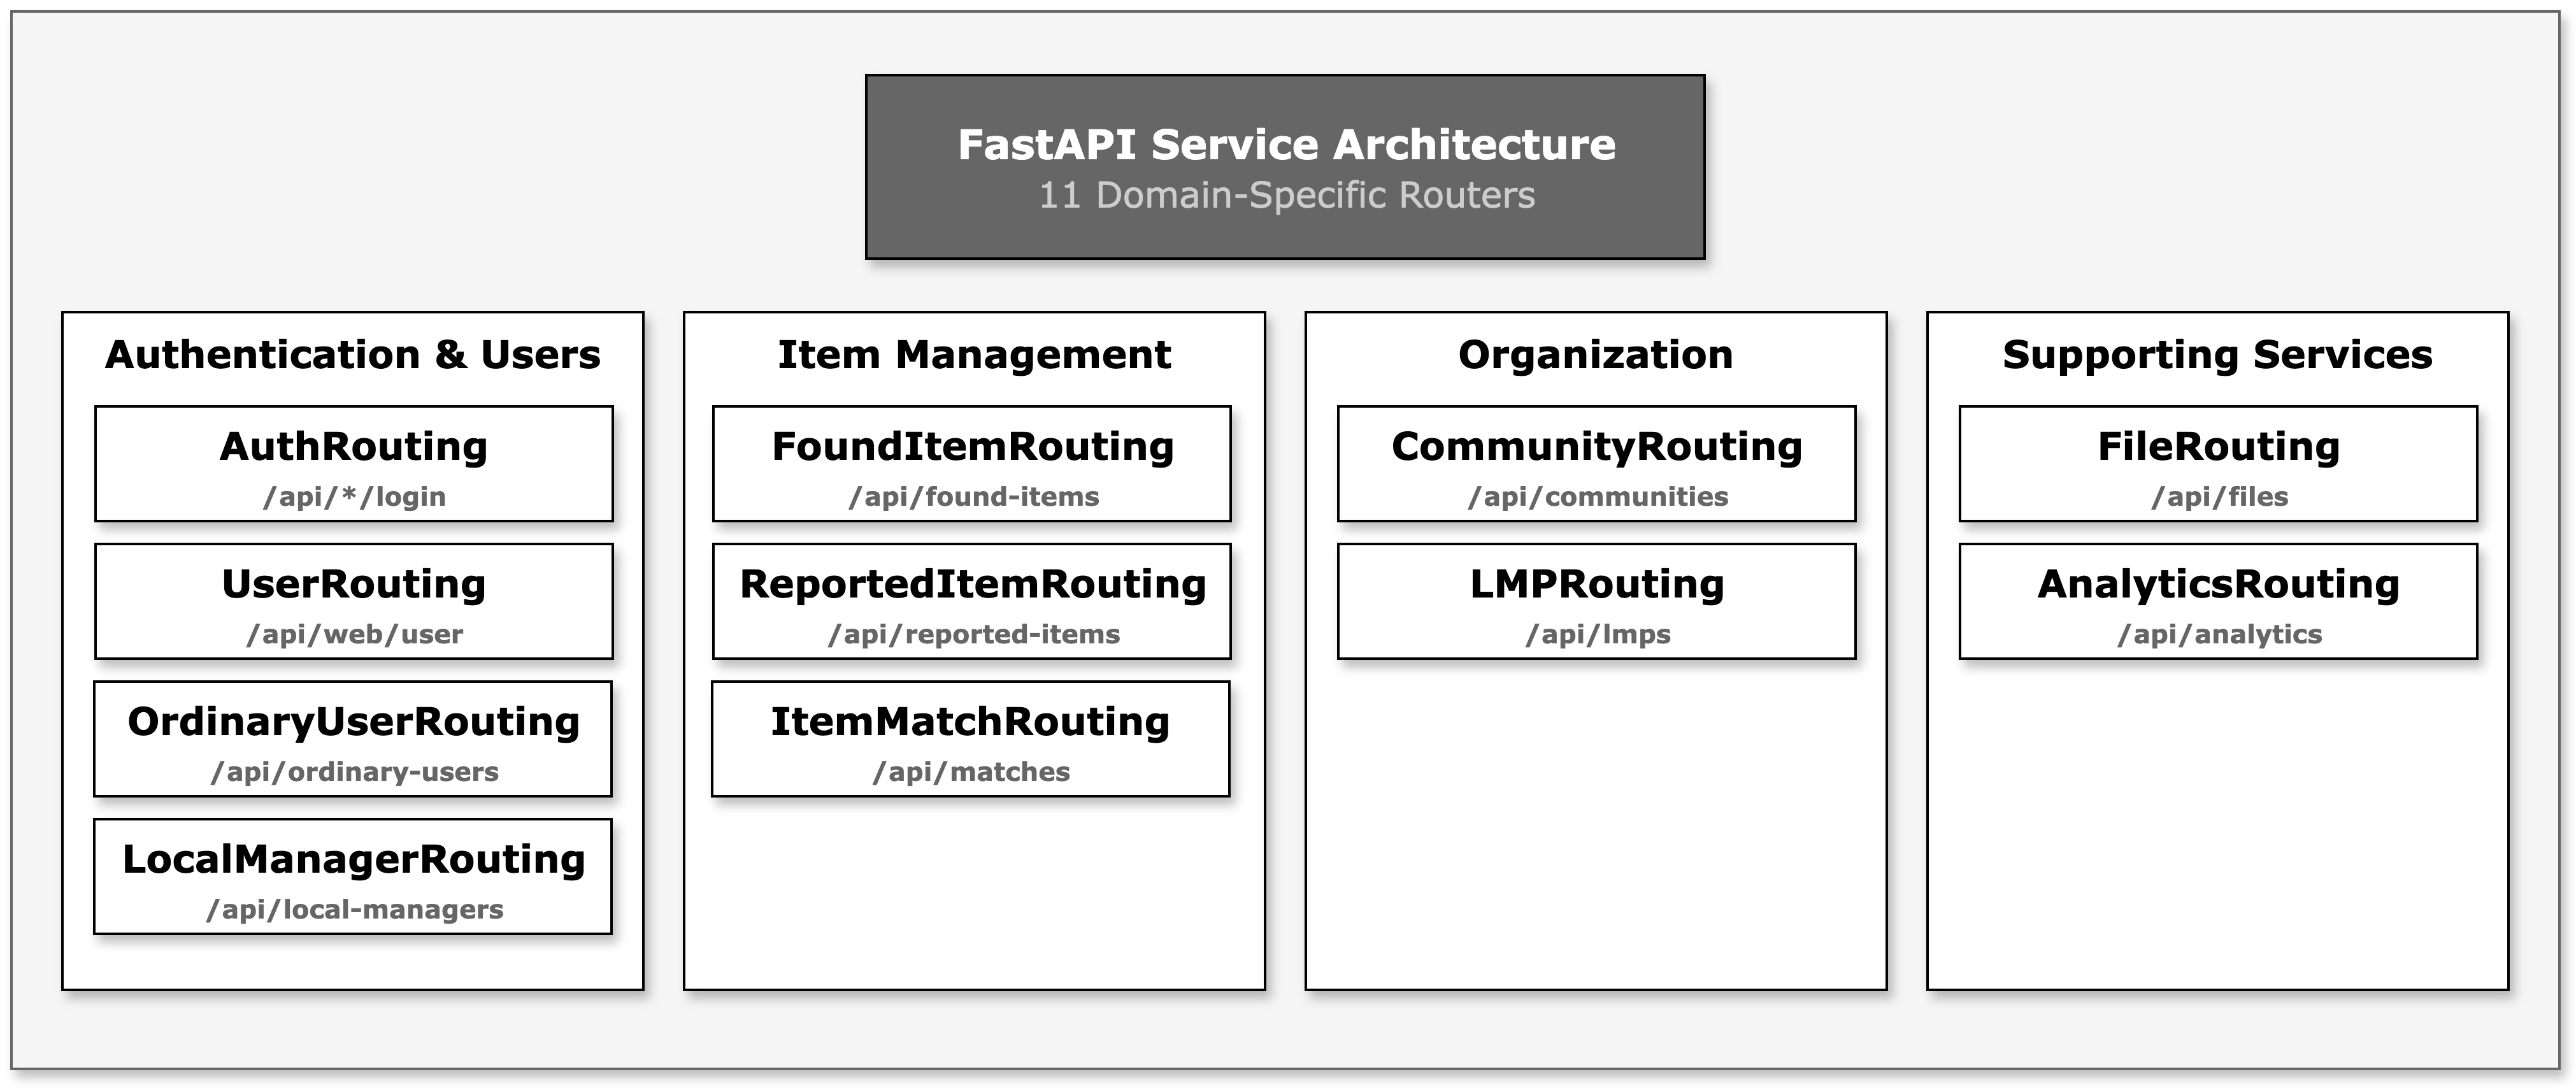
\includegraphics[width=\textwidth]{figs/chapter4/fastapi_routers.png}
    \caption{FastAPI routers architecture showing the 11 domain-specific routers organized into four functional groups: Authentication \& User Management (4 routers), Item Management (3 routers), Organization (2 routers), and Supporting Services (2 routers)}
    \label{fig:fastapi_routers}
\end{figure}

\subsection{Authentication Service Code} \label{subsection:auth_service}

The authentication system distinguishes three user types: ordinary users who access the mobile application, local managers who operate the web dashboard, and system administrators who have full system privileges. Each role maps to a distinct PocketBase collection with specific authentication endpoints. Ordinary users access \texttt{/api/mobile} with public self-registration, while managers and administrators use \texttt{/api/web} with controlled access.

The authentication system validates \acp{jwt} through Base64 \acs{url}-safe decoding and handles automatic refresh with 5-minute expiration thresholds, while in-memory caching provides time-to-live management for improved performance.

Token validation applies a 30-second expiration buffer to determine when tokens should be considered expired, with graceful fallback when refresh attempts fail but tokens remain valid. The system incorporates cleanup mechanisms to prevent memory leaks. Token caching reduces authentication requests to PocketBase during active user sessions.

FastAPI dependencies provide declarative security across \ac{api} endpoints. The user authentication dependency extracts and validates Bearer tokens from request headers, checking the token cache before decoding \ac{jwt} payloads. Role-specific dependencies support both single-role requirements and multiple acceptable roles for flexible access control. Convenience functions handle common administrative patterns and manager-level access requirements. The dependency system creates user authentication objects containing user identifiers, email addresses, collection names, and community associations where applicable. Figure \ref{fig:jwt_auth_sequence} illustrates the complete JWT authentication flow, including token validation, caching mechanisms, and the refresh logic.

\begin{figure}[htbp]
    \centering
    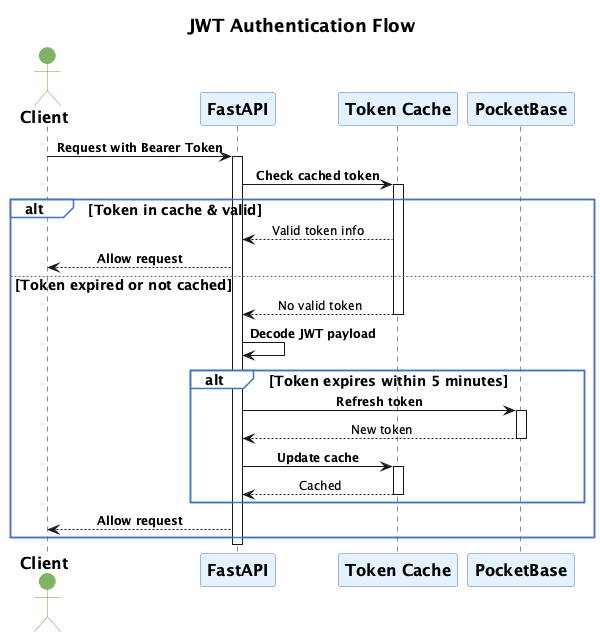
\includegraphics[width=0.8\textwidth]{figs/chapter4/jwt_auth_simple.png}
    \caption{JWT authentication flow showing token validation, caching, and refresh logic with PocketBase integration}
    \label{fig:jwt_auth_sequence}
\end{figure}

\subsection{Item Management Service} \label{subsection:item_management_service}

The item management service orchestrates the complete lifecycle of lost and found items through parallel service implementations that handle both found and reported items with identical architectural patterns. It incorporates intelligent processing capabilities, automated security classification, and asynchronous event handling while maintaining strict community-based access control throughout all operations.

The service architecture provides lifecycle management through retrieval, creation, modification, and deletion operations. When users submit new items, the system validates input data against predefined category enumerations, automatically determines appropriate security levels based on item characteristics, and initiates asynchronous \ac{ai} processing workflows without blocking the main request flow.

The update mechanism implements intelligent re-processing logic that evaluates whether modifications to item properties warrant renewed \ac{ai} analysis. When users modify descriptions or categories - properties that fundamentally affect the matching algorithm - the system automatically requeues items for processing. The query construction system supports suitable filtering capabilities, including fuzzy text matching for flexible search functionality, boolean state filtering for retrieval status tracking, as well as location filtering that considers both delivery points and current storage locations.

\subsubsection{Image Processing and \ac{ai} Integration}

The image processing subsystem uses multimodal \ac{ai} capabilities through the \ac{llava} model to provide automated content analysis and classification. When users upload images, the system generates detailed object descriptions by analysing visual content and automatically assigns appropriate categories through pattern matching against the system's classification taxonomy. To improve performance when handling multiple images simultaneously, the system implements a batch processing strategy that reduces overhead and improves throughput.

\subsubsection{Security Classification and Access Control}

The security framework implements an automated three-tier classification system that analyses item properties to determine appropriate visibility levels. High-security items, including electronics, valuable objects, and other personal documents, receive maximum protection with masked images and obscured descriptions for standard users. Medium-security items, such as bags and sports equipment, maintain image visibility while restricting location details to prevent unauthorised retrieval attempts. Low-security items, including clothing and books, operate with complete transparency, balancing accessibility with reasonable privacy protection.

Access control operates through community-based scoping enforced at the data access layer, so all database operations automatically filter results based on user community membership. \ac{rbac} determines which data fields and operations each user type can access, creating a flexible yet secure authorisation framework.

\subsubsection{Event-Driven Queue Integration}

The queue management system implements a facade pattern that coordinates multiple specialised services handling continuous background processing, batch operations for efficiency, and monitoring capabilities.

When \ac{ai} services become unavailable, the system gracefully degrades to basic functionality while queuing items for later processing. Detailed logging captures operational information for debugging and performance analysis, while structured exception handling maintains clean error propagation through the service components, managing high-throughput processing workloads while preserving data consistency and system stability across operational scenarios.

\subsection{Reverse Proxy Gateway Implementation} \label{subsection:reverse_proxy_gateway}

The system uses a reverse proxy pattern with Nginx rather than a traditional \ac{api} gateway. The design choice favours system simplicity over traditional gateway functionality, creating a single entry point for all services.

The Nginx-based reverse proxy uses path-based routing with static upstream configuration. Request routing follows a clear pattern: \texttt{/api/*} routes to the FastAPI backend on port 8000, \texttt{/pb/*} directs to PocketBase administration on port 8090, and \texttt{/monitoring/*} connects to Grafana dashboards on port 3000. Figure \ref{fig:network_topology} illustrates the complete network topology and routing architecture.

The configuration creates upstream connections with keepalive pools configured for each service type. FastAPI receives 32 keepalive connections for high-throughput \ac{api} operations, while PocketBase administration uses 16 connections for moderate administrative traffic. Connection reuse reduces TCP overhead and improves response times during sustained operation.

\begin{figure}[htbp]
    \centering
    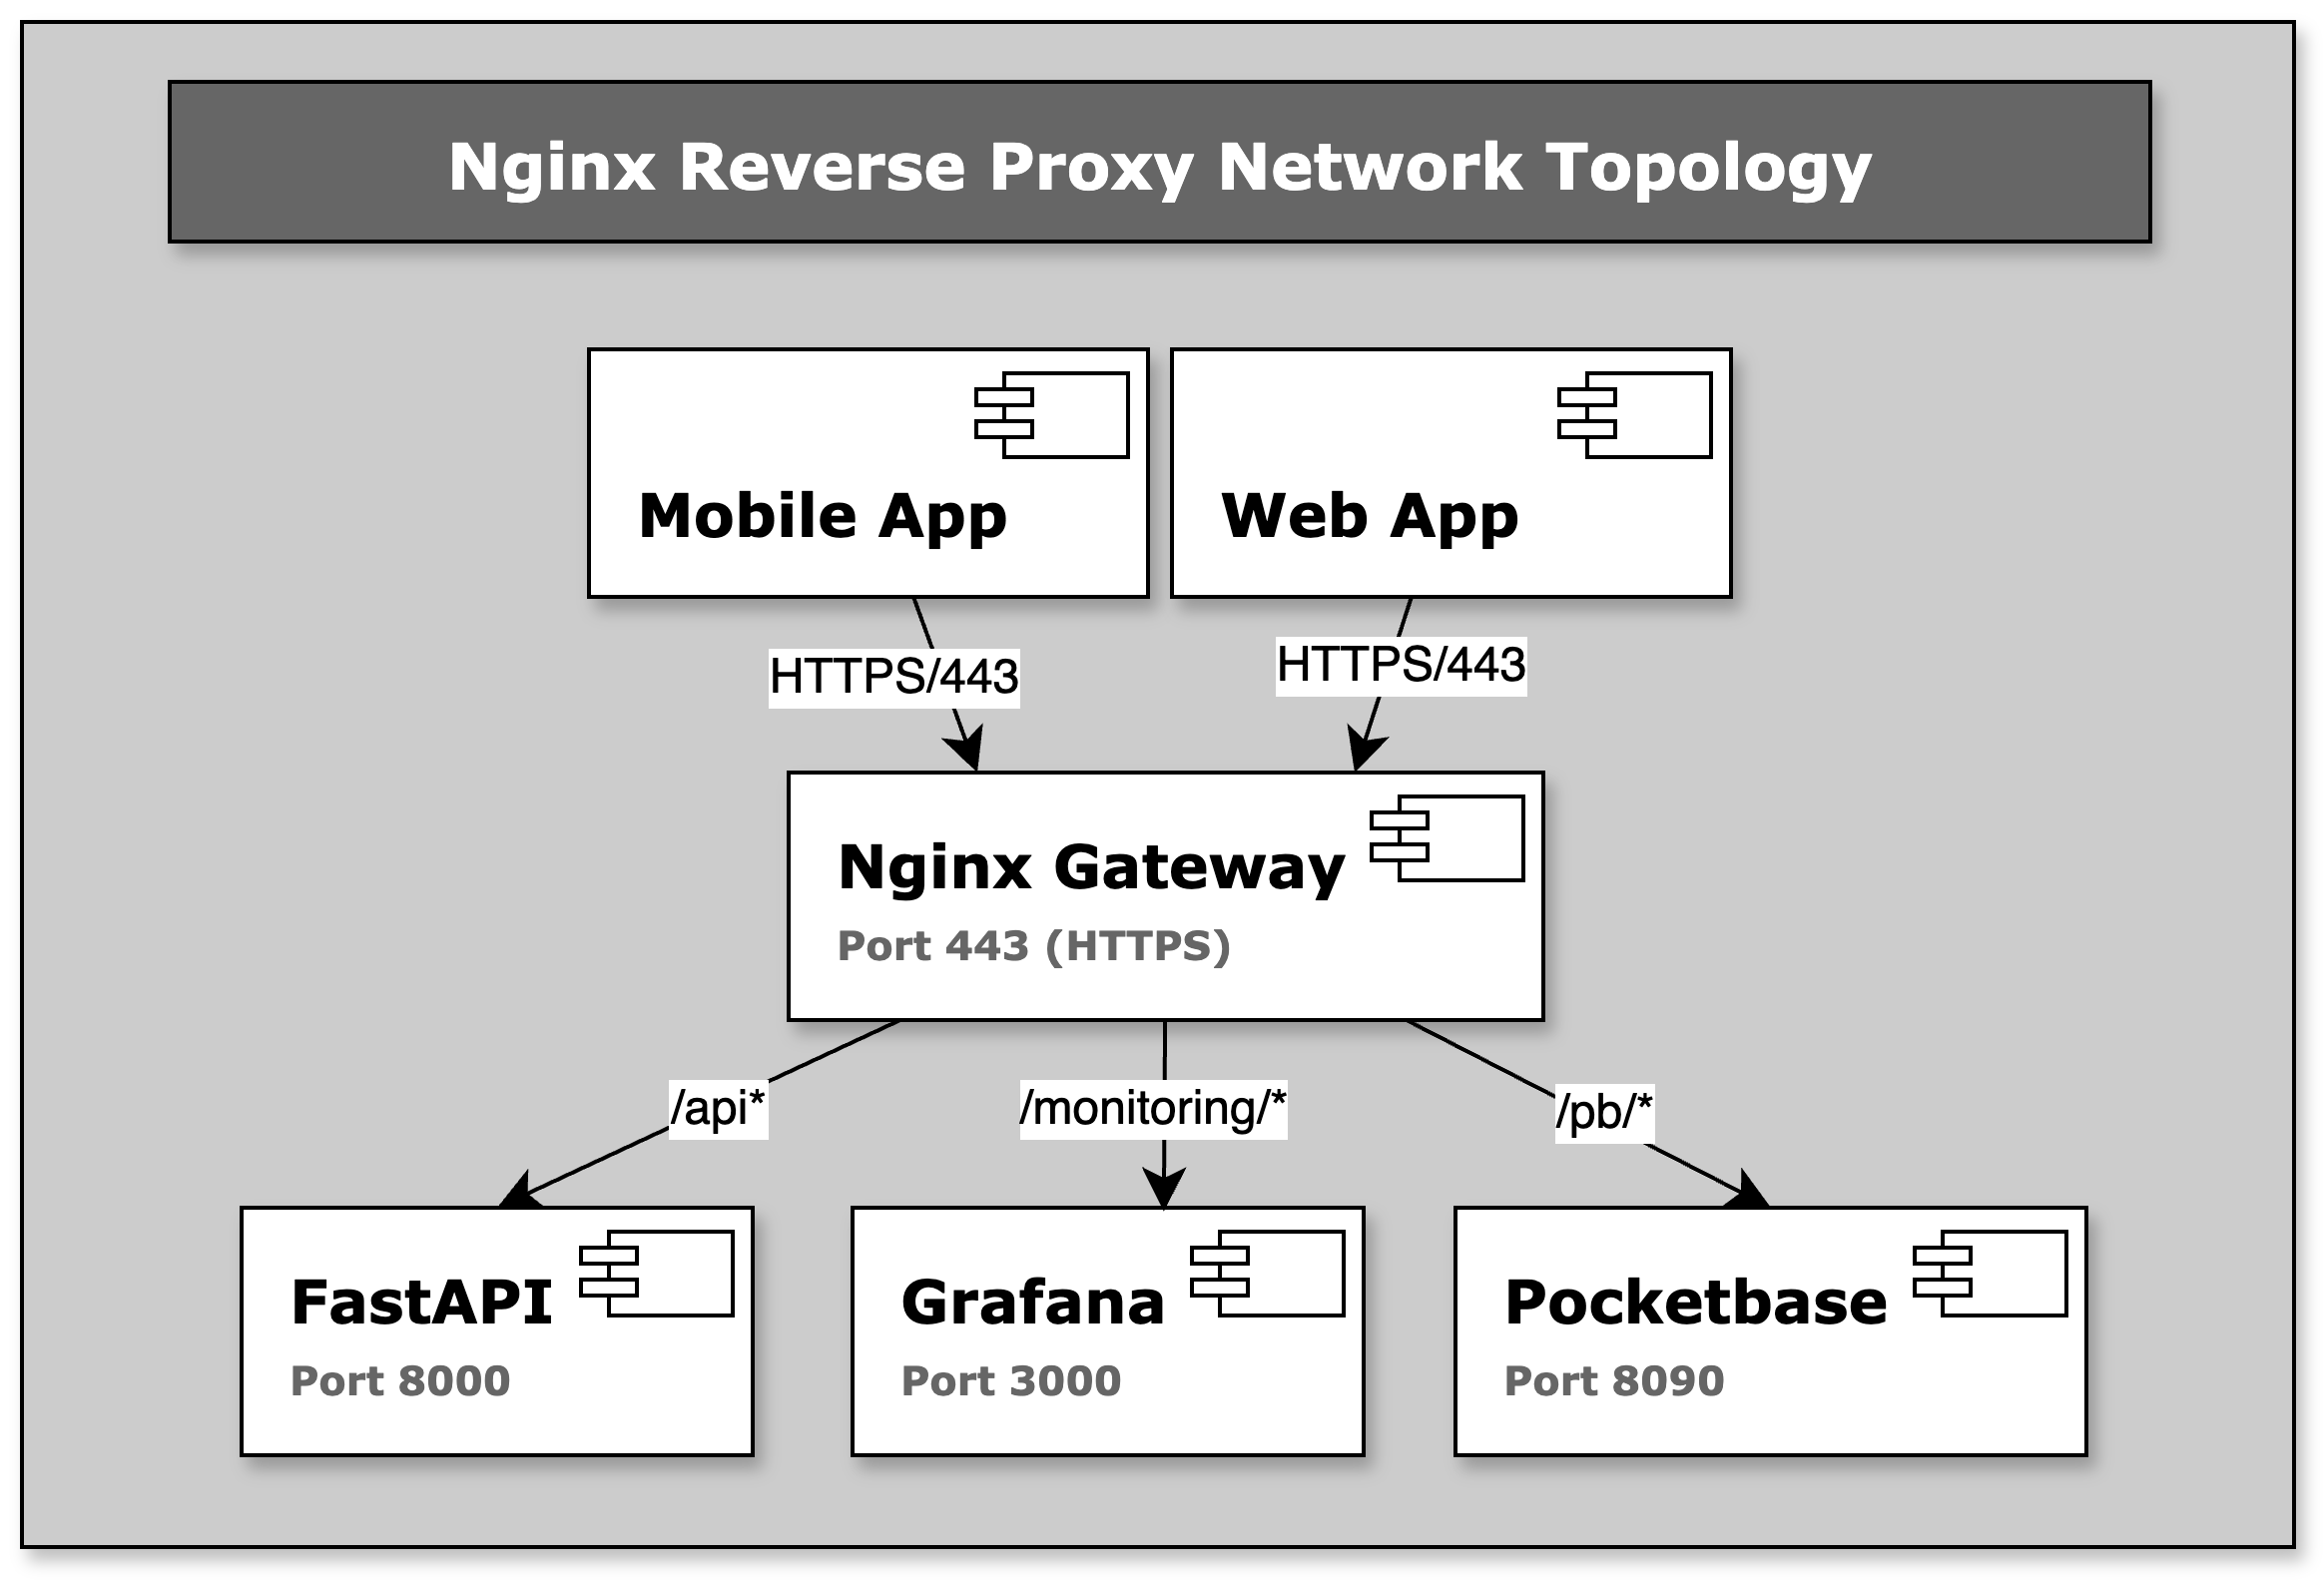
\includegraphics[width=0.5\textwidth]{figs/chapter4/network_topology.png}
    \caption{Network topology diagram showing Nginx reverse proxy routing to backend services with path-based routing, SSL termination, and keepalive connection pools}
    \label{fig:network_topology}
\end{figure}

The reverse proxy enforces \ac{https} redirection with 301\footnote{\url{https://httpstatuses.com/301}} status codes for all \ac{http} requests, securing communication across the system. \ac{ssl} termination occurs at the gateway level, reducing computational overhead on backend services while preserving end-to-end encryption for client communications.

\subsubsection{Authentication Architecture} \label{subsubsection:auth_authorization}

The authentication architecture delegates token validation to the application layer while the gateway handles \ac{ssl} termination and security headers, including \ac{cors} configuration. The gateway does not perform token validation, preserving separation of concerns between infrastructure and application logic. At the application layer, input validation uses Pydantic\footnote{\url{https://docs.pydantic.dev/latest/}} models with email validation following RFC 5322\footnote{\url{https://datatracker.ietf.org/doc/html/rfc5322}} standards, alongside \ac{mime} type restrictions and size limits for file uploads.

\subsubsection{Rate Limiting and Throttling} \label{subsubsection:rate_limiting}

The Nginx configuration applies differentiated rate limiting based on endpoint functionality and security requirements. Considering system protection with standard application usage patterns, \ac{api} endpoints enforce 60 requests per minute with burst capacity of 20 requests. Authentication endpoints apply stricter limits of 10 requests per minute with 5-request bursts to prevent credential-based attacks, such as brute force attempts.

File upload functions receive 20 requests per minute with 10-request bursts, accounting for the time-intensive nature of image processing while preventing abuse. Administrative interfaces implement the most restrictive limits: 5 requests per minute with configurable burst capacity. The limits were designed to accommodate legitimate use cases incorporated in the application and to block abusive patterns. Table \ref{tab:rate_limiting_config} summarizes the complete rate limiting configuration across all endpoint types.

Connection limiting complements request rate limiting by restricting concurrent connections per \ac{ip} address. \ac{api} operations allow up to 10 concurrent connections per \ac{ip}. At the same time, authentication endpoints limit connections to 3 per \ac{ip}, preventing connection exhaustion attacks while accommodating legitimate multi-tab browsing and mobile application usage.

Rate limiting uses Nginx's \texttt{limit\_req} and \texttt{limit\_conn} modules with memory-based storage for fast enforcement without external dependencies. Rate limit violations return 429\footnote{\url{https://httpstatuses.com/429}} status codes with appropriate error messages, allowing client-side retry logic and clearly communicating the limitation to \ac{api} consumers. Figure \ref{fig:rate_limiting_effectiveness} demonstrates the effectiveness of these rate limiting measures in protecting the system from abusive traffic patterns.

\begin{table}[htbp]
    \centering
    \caption{Rate limiting configuration by endpoint type with request limits and burst capacities}
    \label{tab:rate_limiting_config}
    \begin{tabular}{@{}llll@{}}
        \toprule
        \textbf{Endpoint Type} & \textbf{Rate Limit} & \textbf{Burst Capacity} & \textbf{Connection Limit} \\
        \midrule
        General \ac{api} & 60 requests/min & 20 requests & 10 connections \\
        Authentication & 10 requests/min & 5 requests & 3 connections \\
        File Upload & 20 requests/min & 10 requests & 5 connections \\
        PocketBase Admin & 5 requests/min & 3 requests & 2 connections \\
        Grafana Monitoring & 5 requests/min & 5 requests & 2 connections \\
        \bottomrule
    \end{tabular}
\end{table}

\begin{figure}[htbp]
    \centering
    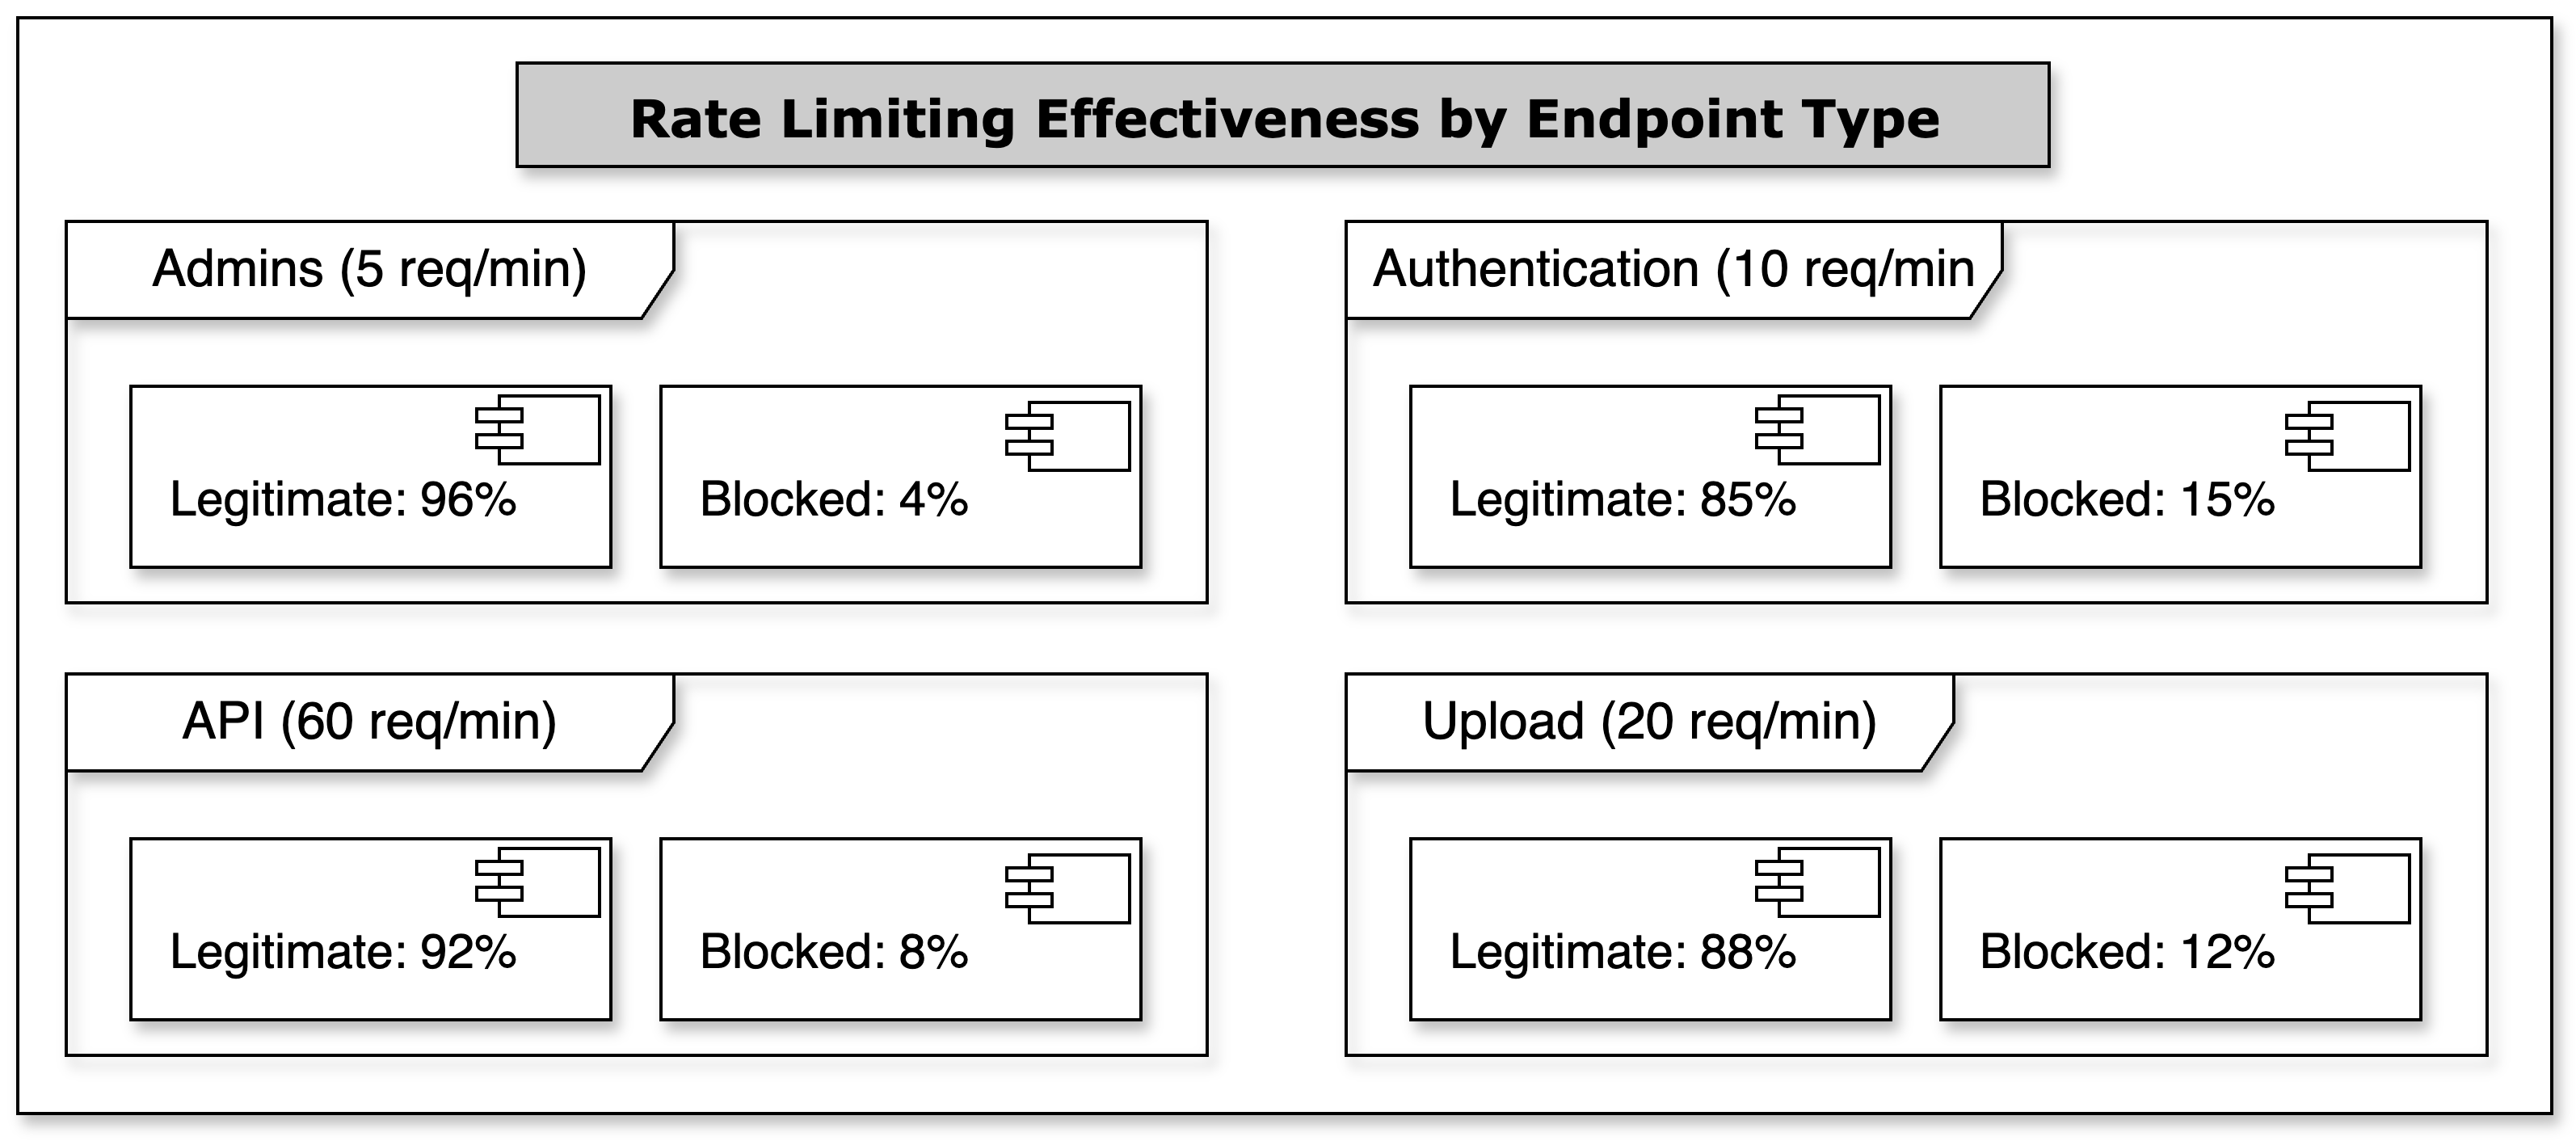
\includegraphics[width=0.75\textwidth]{figs/chapter4/rate_limiting_chart.png}
    \caption{Rate limiting effectiveness metrics showing request blocking rates and system protection across different endpoint types}
    \label{fig:rate_limiting_effectiveness}
\end{figure}

\subsection{Community and Location Services} \label{subsection:community_location_services}

The community and location services establish the organisational foundation and geographic intelligence capabilities that enable multi-tenant operation and location-aware matching. This module manages hierarchical relationships between users, communities, and physical collection points while providing geographic calculations for proximity-based item matching.

\subsubsection{Community Management Architecture}

The community management system implements organisational control, handling the relationships and permissions that define the multi-tenant architecture. It provides role-aware access patterns where system administrators can manage their assigned communities with full administrative capabilities, local managers access communities through their associated managing points with operational permissions, and ordinary users participate in multiple communities based on their membership associations. Administrative operations support community configuration updates, including visual identity management through avatar uploads and ownership transfer with appropriate validation safeguards.

The system manages user-community associations through a dedicated service module that handles the many-to-many relationships between ordinary users and their communities. The architecture enables efficient retrieval of all members within a specific community for administrative oversight, while also supporting user-centric queries to determine an individual's community memberships. The temporal dimension of these relationships is preserved through timestamp tracking, which is recorded when users join communities for audit and analysis purposes. The implementation utilises database expansion capabilities to retrieve complete relationship graphs in a single operation, improving performance for organisational queries.

\subsubsection{Local Managing Points Implementation}

Physical collection and distribution points are managed through a specialised service that combines location management with geospatial intelligence capabilities. When establishing new managing points, the system processes geographic coordinates as structured data containing precise latitude and longitude information, handles image uploads for visual identification of physical locations, and validates community associations to maintain proper organisational boundaries. The implementation supports flexible data retrieval with configurable pagination ranging from single-item queries to bulk operations processing up to 100,000 records. At the same time, relationship expansion capabilities allow selective loading of related data based on performance requirements.

Modification operations support partial updates to managing point configurations, enabling changes to geographic coordinates when facilities relocate and image updates for refreshed visual identification.

\subsubsection{Geographic Distance Calculations}

The location calculation service implements geographic algorithms that power the system's proximity-based matching capabilities. Distance calculations employ the Haversine formula \cite{Sinnott1984} to compute great circle distances between coordinate pairs, providing accurate measurements that account for the Earth's spherical geometry. The system categorises distances using configurable thresholds that define proximity bands: very close for items within 1 kilometre, close for 5-kilometre ranges, moderate for 20-kilometre distances, and far for separations up to 100 kilometres.

Distance measurements are transformed into normalised proximity scores through a scaling algorithm that applies linear interpolation for nearby items and logarithmic decay for distant objects. This makes minor distance differences matter more for nearby items while still considering distant matches when relevant. The coordinate extraction system processes location data from multiple sources and formats, integrating geographic information into the \ac{ai} matching pipeline for location-aware item pairing decisions.


% ____________________ AI Integration and Matching Implementation ____________________ %

\section{\ac{ai} Integration and Matching Implementation} \label{section:ai_integration}

\subsection{\ac{llava} Client Implementation} \label{subsection:llava_client}

The \ac{llava} client provides multimodal \ac{ai} capabilities through integration with Ollama server infrastructure, combining text and image analysis for automated item description generation and visual similarity matching.

\subsubsection{Ollama Integration Architecture}

The \ac{llava} client connects to the remote Ollama server using Bearer token authentication with \ac{jwt} format credentials. The implementation underwent critical fixes during development, transitioning from broken \texttt{ollama.generate} imports to proper \texttt{ollama.Client()} instantiation with correct authentication headers.


The client configuration includes host specification via environment variables, authorisation headers for secure communication, and connection parameters configured for different analysis types. Text analysis uses a 2048 token context with 30-second timeouts and a temperature of 0.1 for consistent results, while image analysis extends to a 4096 token context with 45-second timeouts to accommodate visual processing requirements.

\subsubsection{Multimodal Analysis Implementation}

The filing service coordinates \ac{ai}-powered image analysis using the prompt "Describe the main central object in this image..." for automatic description generation. Category assignment operates through object matching against the complete classification taxonomy, with fallback to a general category when classification confidence proves insufficient.

Image processing includes PNG\footnote{\url{https://en.wikipedia.org/wiki/Portable_Network_Graphics}} conversion and validation for \ac{ai} compatibility, providing consistent input formats for reliable analysis. The service implements batch file operations to improve performance during multiple image retrievals, while validation error handling prevents system interruptions when \ac{ai} services become temporarily unavailable.

\subsection{Matching Algorithm Implementation} \label{subsection:matching_algorithm}

The matching algorithm uses a multi-factor scoring system that combines the previously mentioned factors (semantic understanding, visual analysis, geographic and temporal proximity, and contextual relevance) to identify potential item matches, using \ac{ai}-powered comparison across multiple dimensions while maintaining the performance characteristics necessary for real-time operational requirements.

\subsubsection{Multi-Factor Scoring Architecture}

The confidence calculation implements a carefully calibrated weighted algorithm that balances different matching factors based on their empirical predictive value. Description similarity represents the most significant factor at 40\% weight, utilising semantic text analysis to understand meaning beyond simple keyword matching. Category alignment contributes 25\% to the overall score, recognising that correct classification provides strong correlation signals. Visual similarity through multimodal image comparison accounts for 20\% of the score, offering crucial confirmation when textual descriptions may vary. Geographic proximity adds 10\% weight to favour nearby matches while still considering distant possibilities, and temporal relevance contributes the final 5\% to acknowledge the correlation between report and discovery timing.

The scoring architecture normalises each factor to a standard 0.0 to 1.0 scale before applying weights, providing balanced contributions regardless of the underlying measurement scales.

Figure \ref{fig:ai_scoring_system} illustrates the distribution of weighted scoring factors and the binary confidence threshold system that determines user interactions.

\begin{figure}[htbp]
    \centering
    \begin{subfigure}[t]{0.48\textwidth}
        \centering
        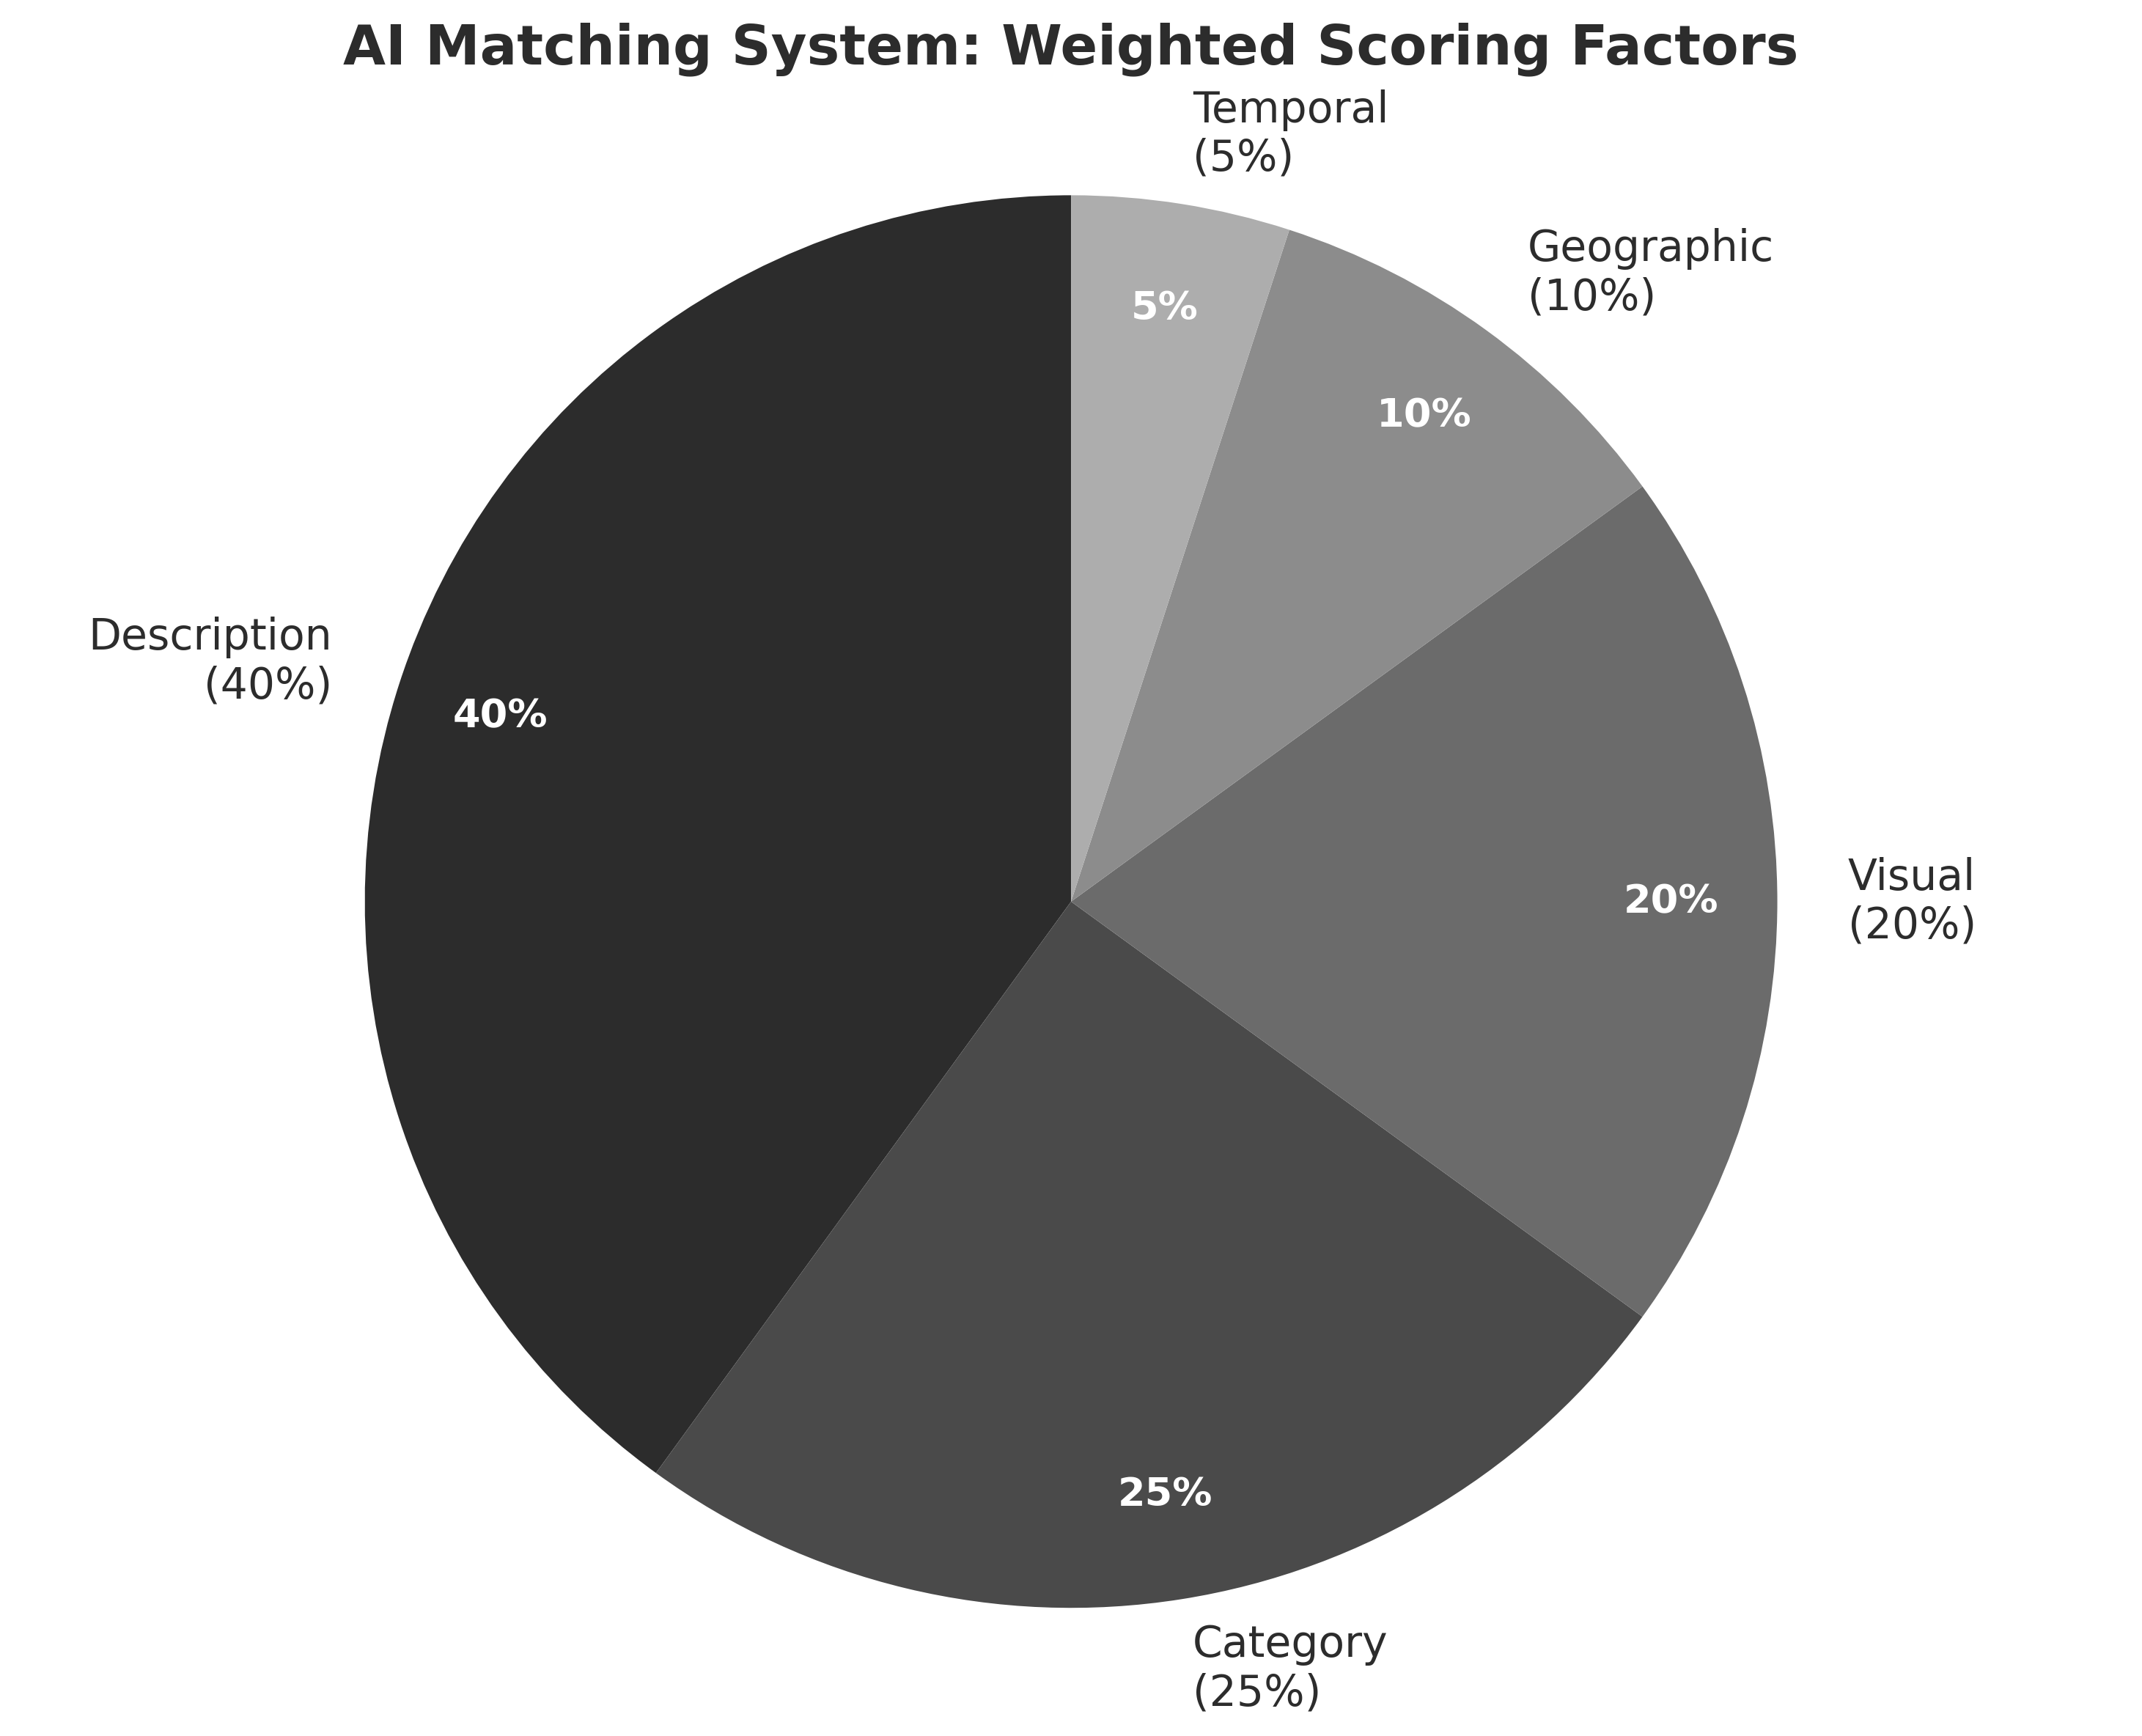
\includegraphics[width=\textwidth]{figs/chapter4/scoring_factors_chart.png}
        \caption{Weighted scoring factors distribution}
        \label{fig:scoring_factors}
    \end{subfigure}
    \hfill
    \begin{subfigure}[t]{0.48\textwidth}
        \centering
        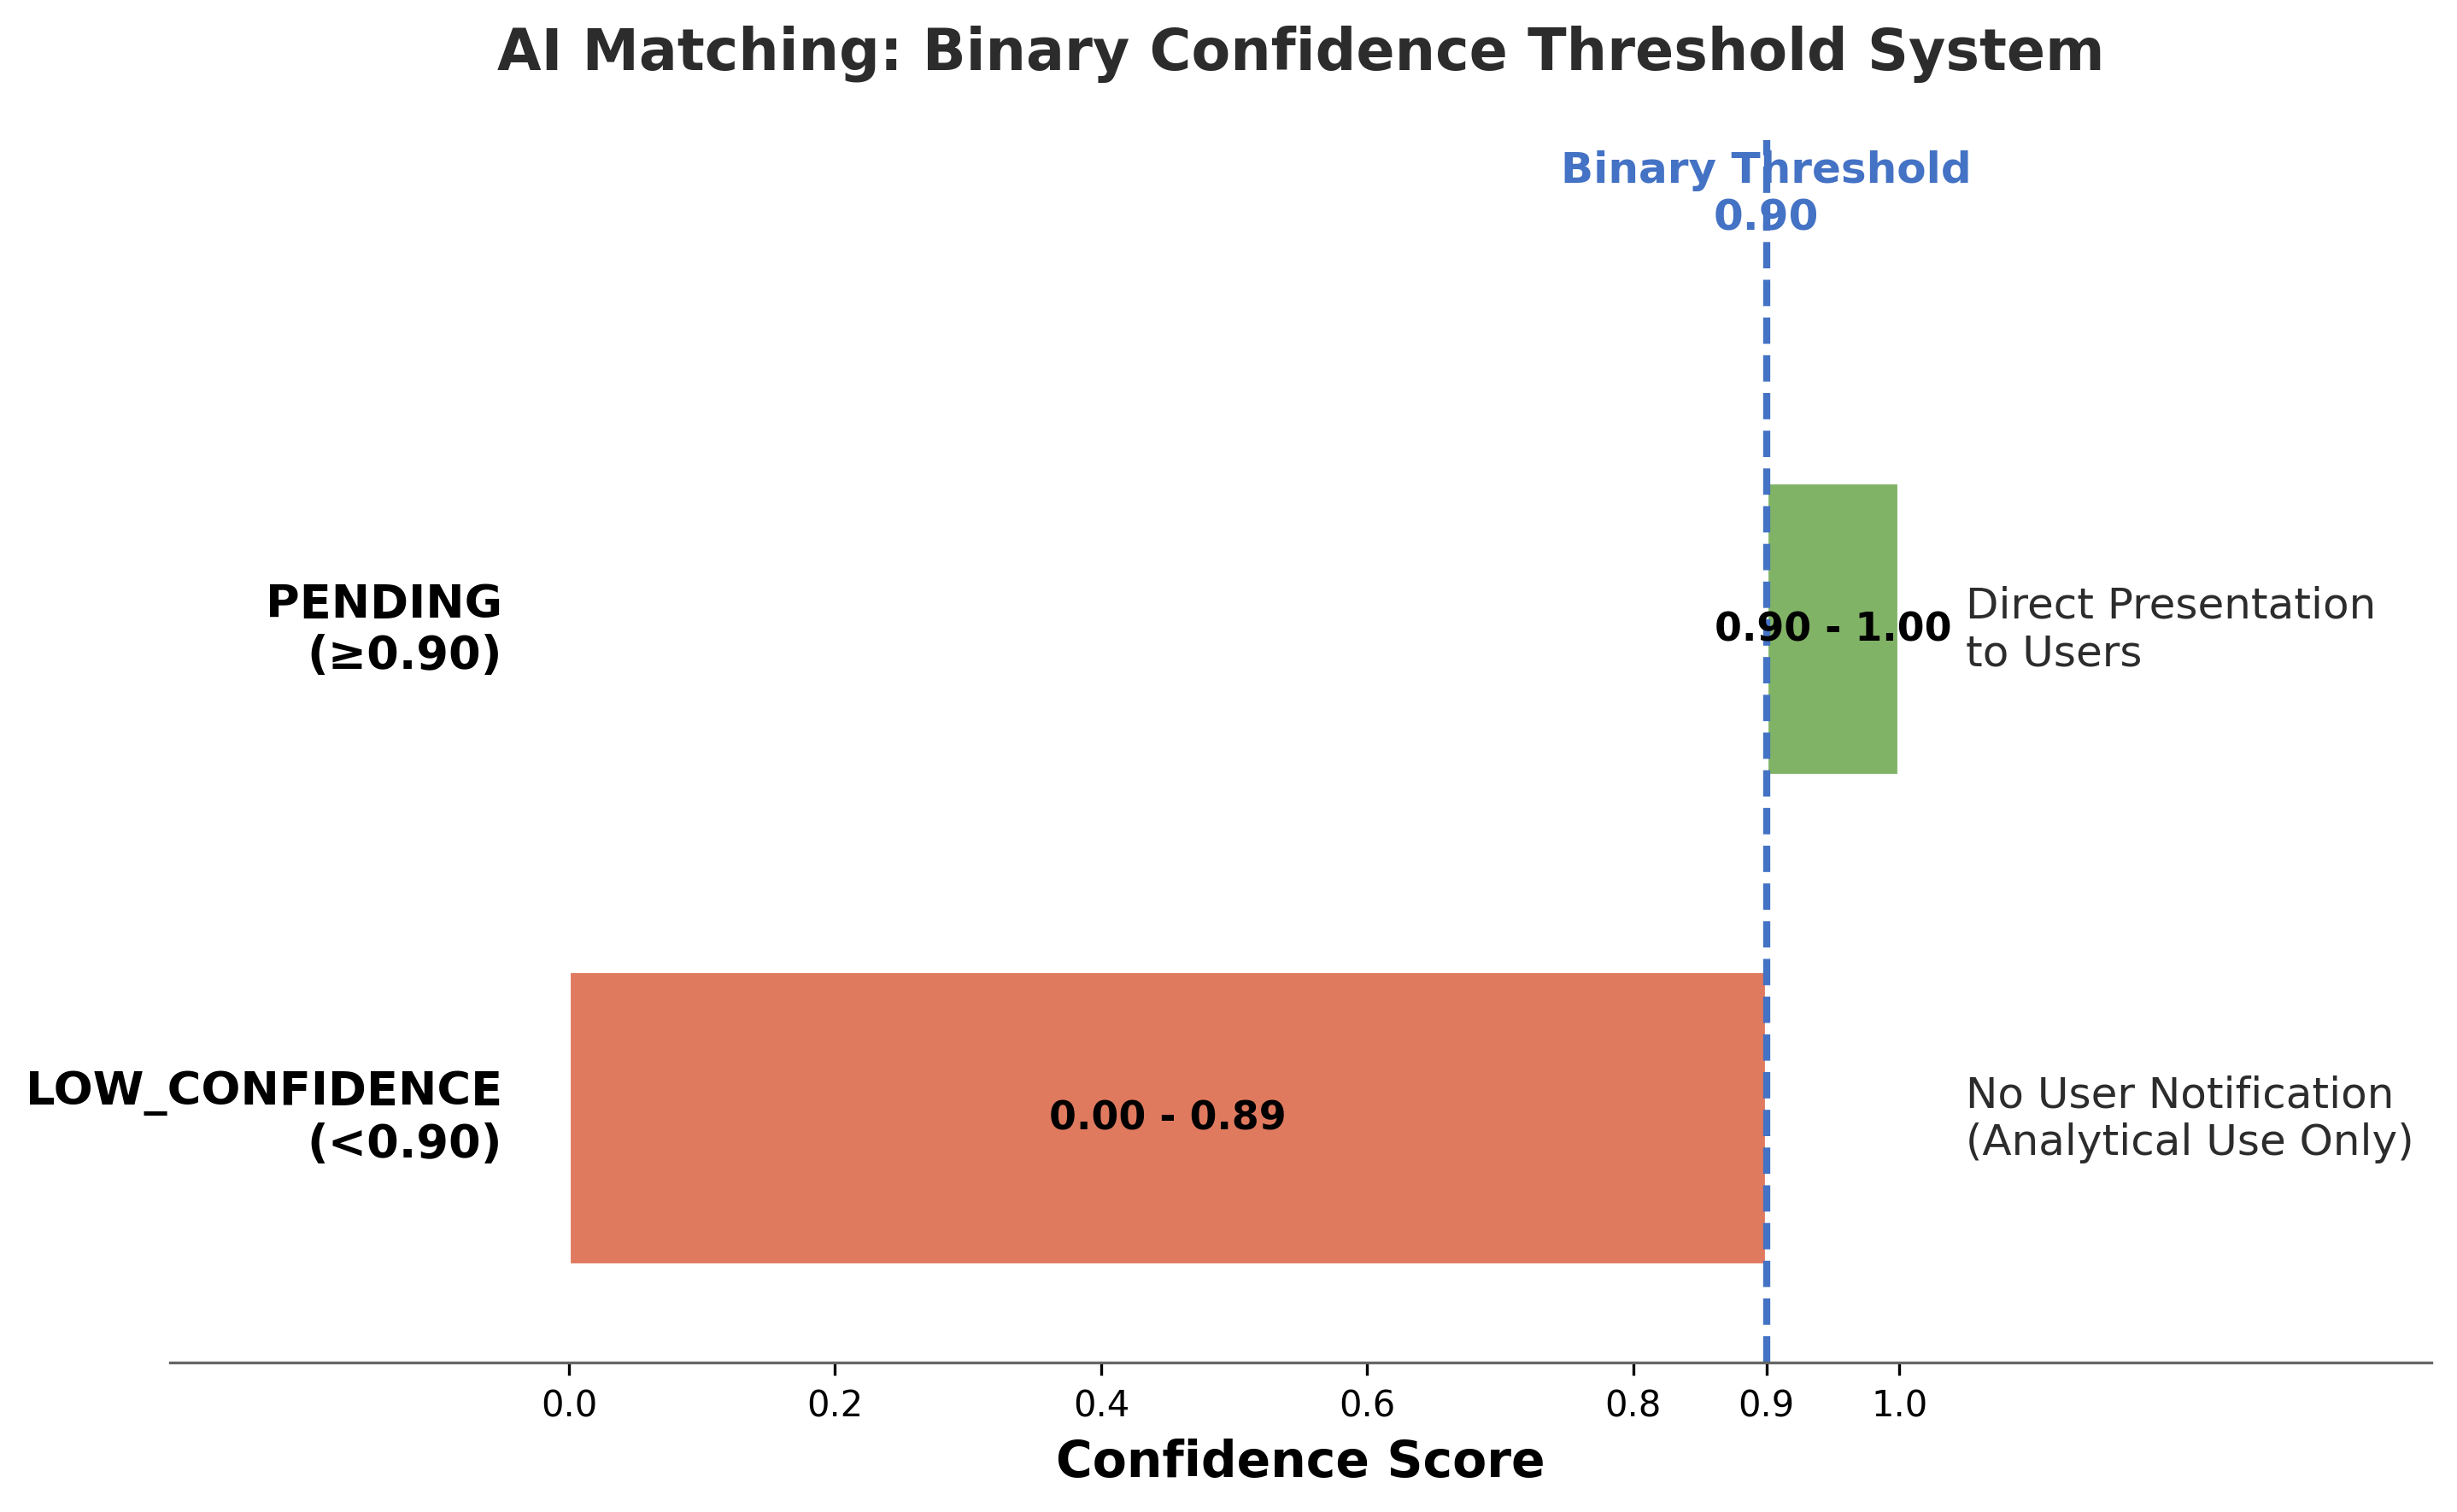
\includegraphics[width=\textwidth]{figs/chapter4/confidence_bands_chart.png}
        \caption{Binary confidence threshold and user interactions}
        \label{fig:confidence_bands}
    \end{subfigure}
    \caption{Scoring system}
    \label{fig:ai_scoring_system}
\end{figure}

\subsubsection{Confidence Threshold Management}

The system implements a binary confidence threshold at 0.90 that determines how users interact with potential matches. Matches achieving confidence scores at or above 0.90 are classified as \texttt{PENDING} status and presented to users as highly probable reunifications, requiring only minimal verification before confirmation. Matches scoring below 0.90 are classified as \texttt{LOW\_CONFIDENCE} status and are excluded from immediate user notification to prevent notification fatigue, though the system retains these matches for analytical purposes and algorithm improvement.

The binary threshold system balances maximising successful reunifications while minimising false positive notifications that could undermine user trust. This approach provides clear operational boundaries and reduces complexity in both implementation and user experience.



\subsection{Queue Processing Implementation} \label{subsection:queue_processing}

The queue processing system manages asynchronous item processing operations through a service-oriented architecture that balances continuous background processing and batch operations.

The queue management system implements a facade pattern that coordinates four specialised services, each designed for specific operational requirements. The continuous processing service maintains persistent background operations with sleep and backoff mechanisms that adapt to workload variations, maximising overall throughput by maintaining constant operation with minimal idle time. The batch processing service manages community-specific operations with configurable batch sizes that balance throughput and resource utilisation, improving performance through grouping and resource pooling. Administrative capabilities are provided through a dedicated management service that enables queue manipulation and manual intervention when necessary, prioritising reliability and data consistency over raw performance. Real-time monitoring delivers statistics and health assessments that inform operational decisions and capacity planning, providing observability without impacting processing performance. The services share common interfaces and error handling patterns, but maintain operational independence.

\subsubsection{Batch Processing and Workflow Management}

The batch processing implementation groups items by community to provide fair resource allocation across the multi-tenant architecture. Processing cycles handle up to 10 items per community. The system implements adaptive timing strategies with 5-second delays between active processing cycles to prevent resource exhaustion, extending to 30-second idle periods when queues are empty to reduce unnecessary computational overhead.

Workflow management tracks item progression through clearly defined states that enable precise monitoring and error recovery. Items enter the queue in a pending state and are awaiting their processing turn. The processing state indicates active \ac{ai} analysis in progress, preventing duplicate processing attempts. Completed and failed states represent terminal conditions that trigger appropriate follow-up actions. State transitions employ atomic operations wherever the underlying database supports them, with carefully designed compensating actions for multi-step processes that cannot be completed atomically within the database's transactional constraints.

\subsubsection{Error Handling and Recovery Mechanisms}

The queue system distinguishes between transient and permanent failures. Transient failures trigger exponential backoff retry mechanisms with gradually increasing delay intervals, while permanent failures are immediately marked and removed from active processing to prevent queue blockage. State tracking with unique identifiers and timestamps prevents duplicate processing during system restarts, enabling operations to resume exactly where interruptions occurred.

\subsubsection{Monitoring Infrastructure}

The monitoring infrastructure provides real-time visibility into queue operations through detailed metrics collection. The system tracks throughput with community-level granularity, latency across different processing stages, and success rates broken down by community and item type. The monitoring implementation integrates with Prometheus and Grafana for metrics collection, visualisation, and alerting capabilities, automatically tracking request latency, response patterns, and system resource utilisation with configurable alerting for threshold violations.

The matching algorithm performance analysis reveals distinct characteristics between high-confidence and low-confidence matches. Figure \ref{fig:ai_matching_system} demonstrates the accuracy rates achieved for each confidence level and shows the corresponding processing time requirements.

\begin{figure}[htbp]
    \centering
    \begin{subfigure}[t]{0.48\textwidth}
        \centering
        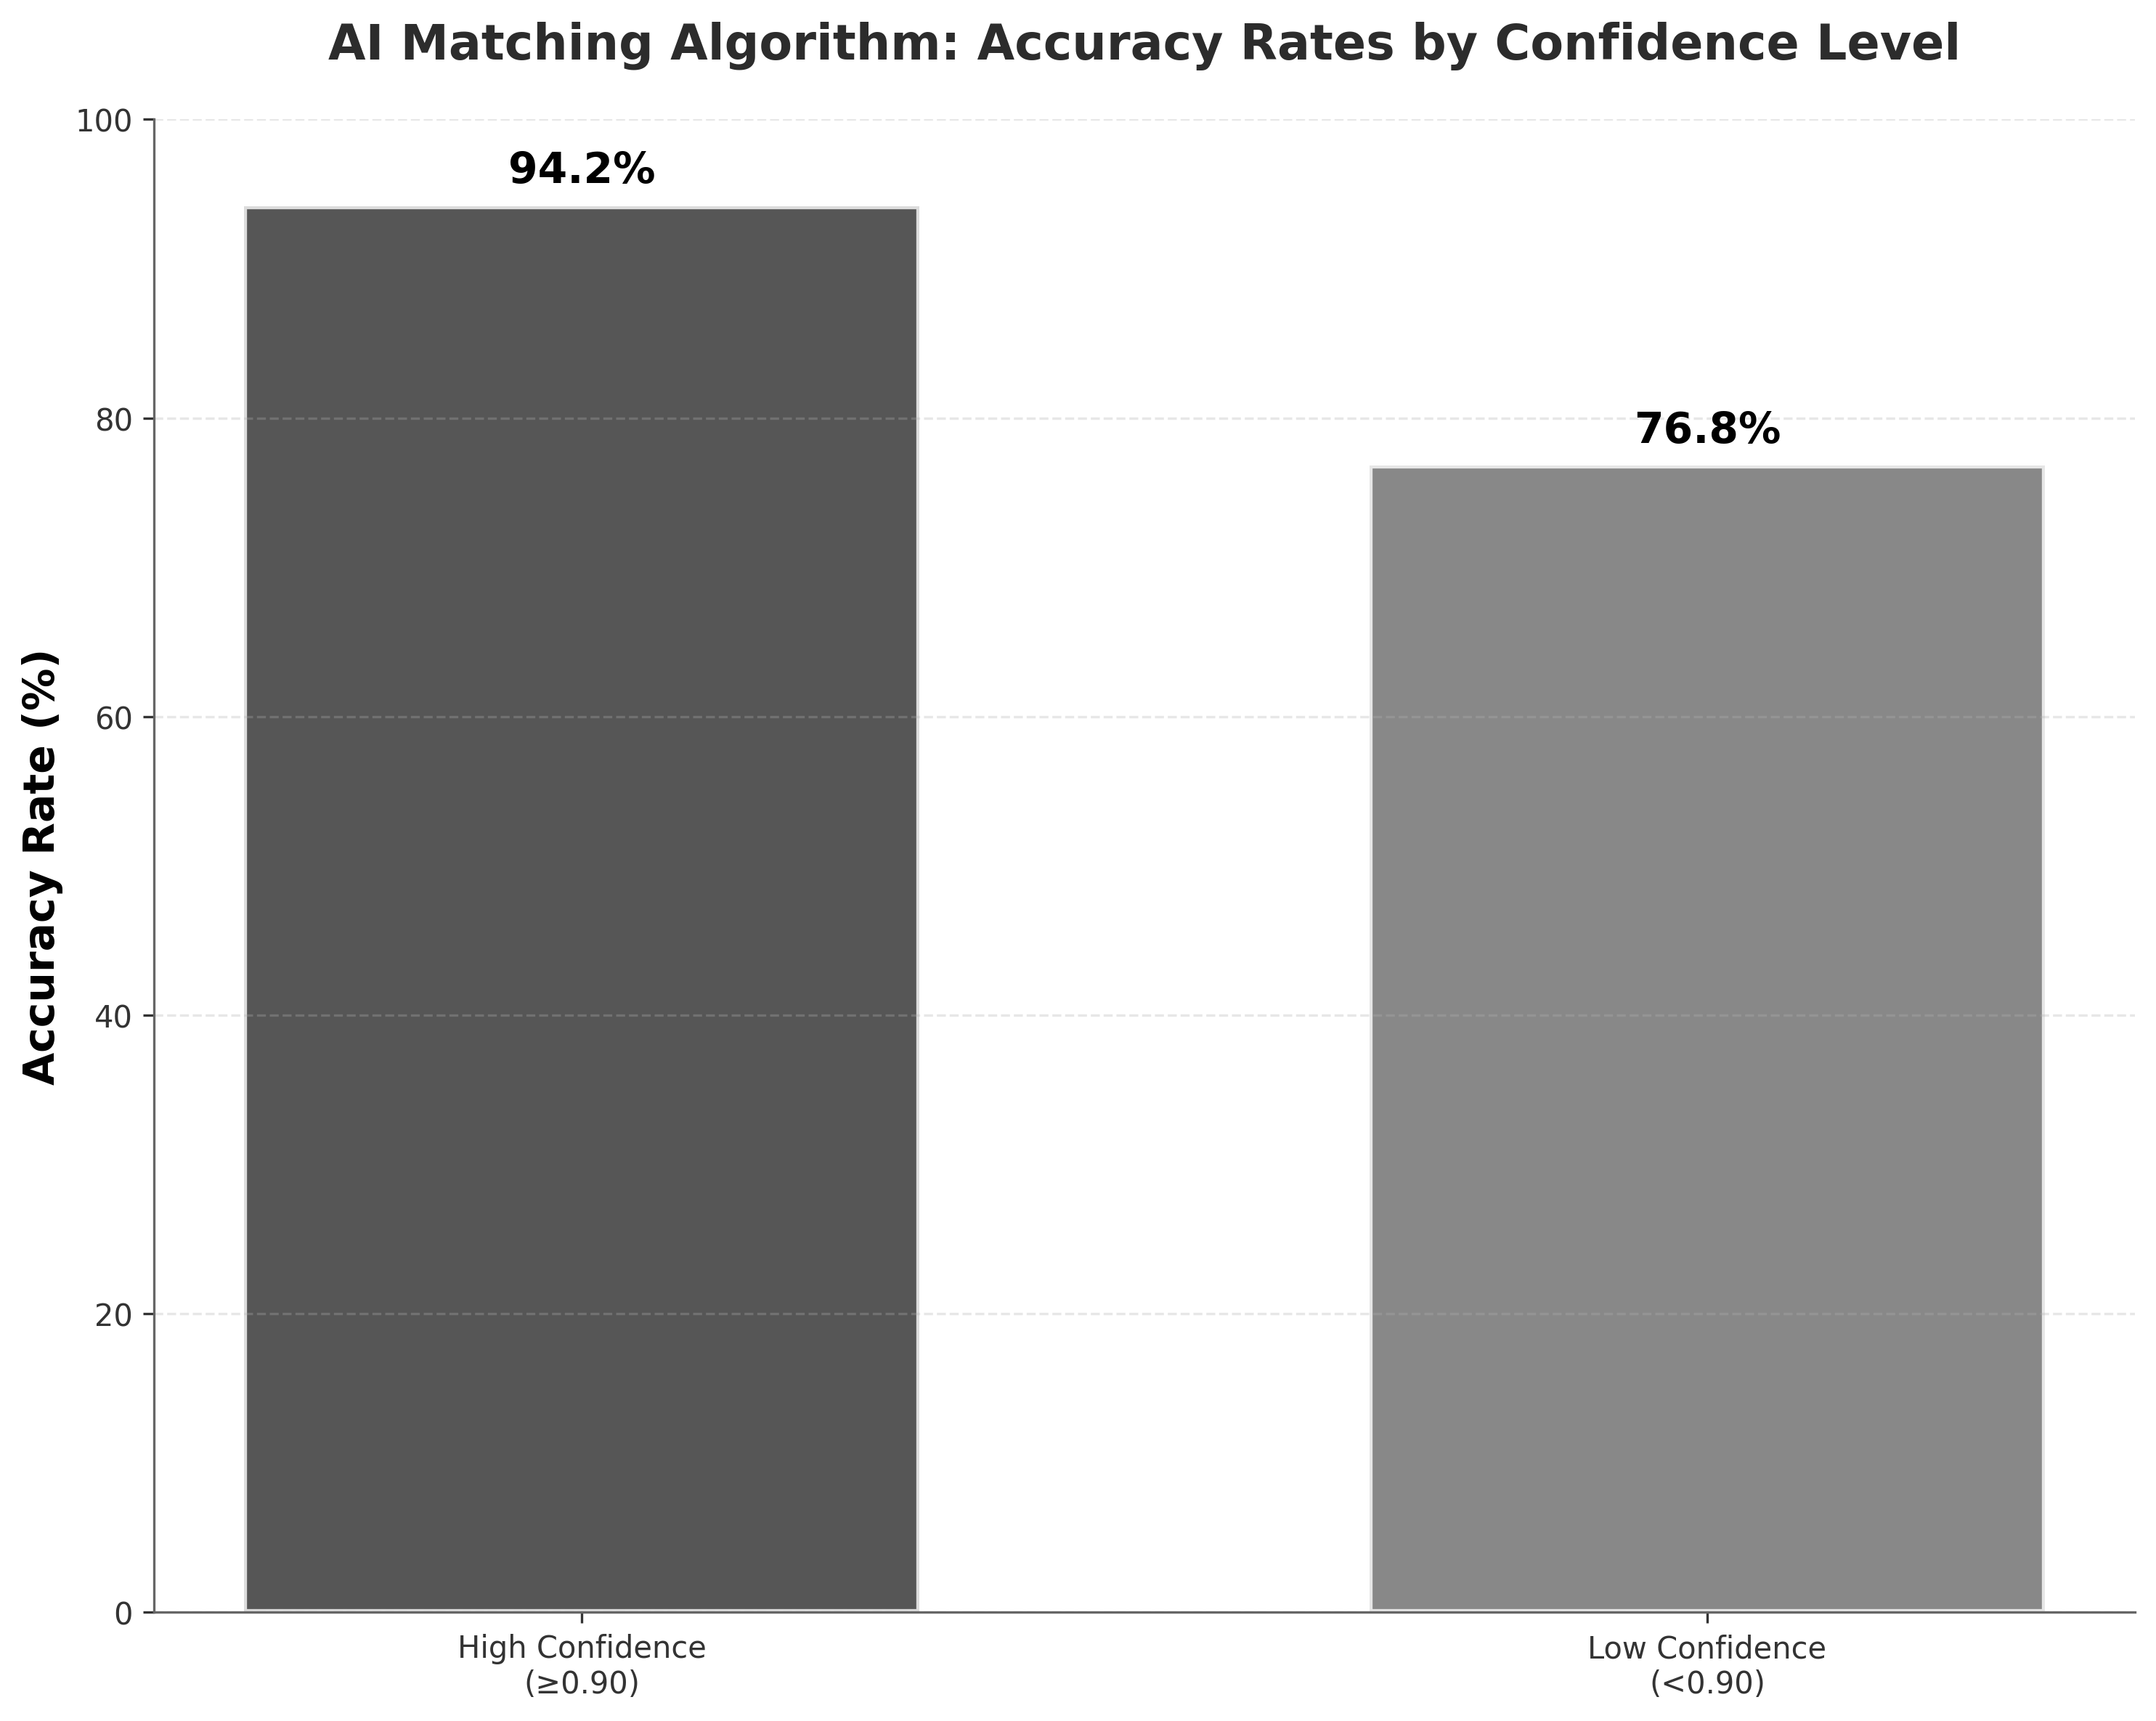
\includegraphics[width=\textwidth]{figs/chapter4/ai_accuracy_rates.png}
        \caption{AI Matching Algorithm: Accuracy Rates by Confidence Level}
        \label{fig:ai_accuracy}
    \end{subfigure}
    \hfill
    \begin{subfigure}[t]{0.48\textwidth}
        \centering
        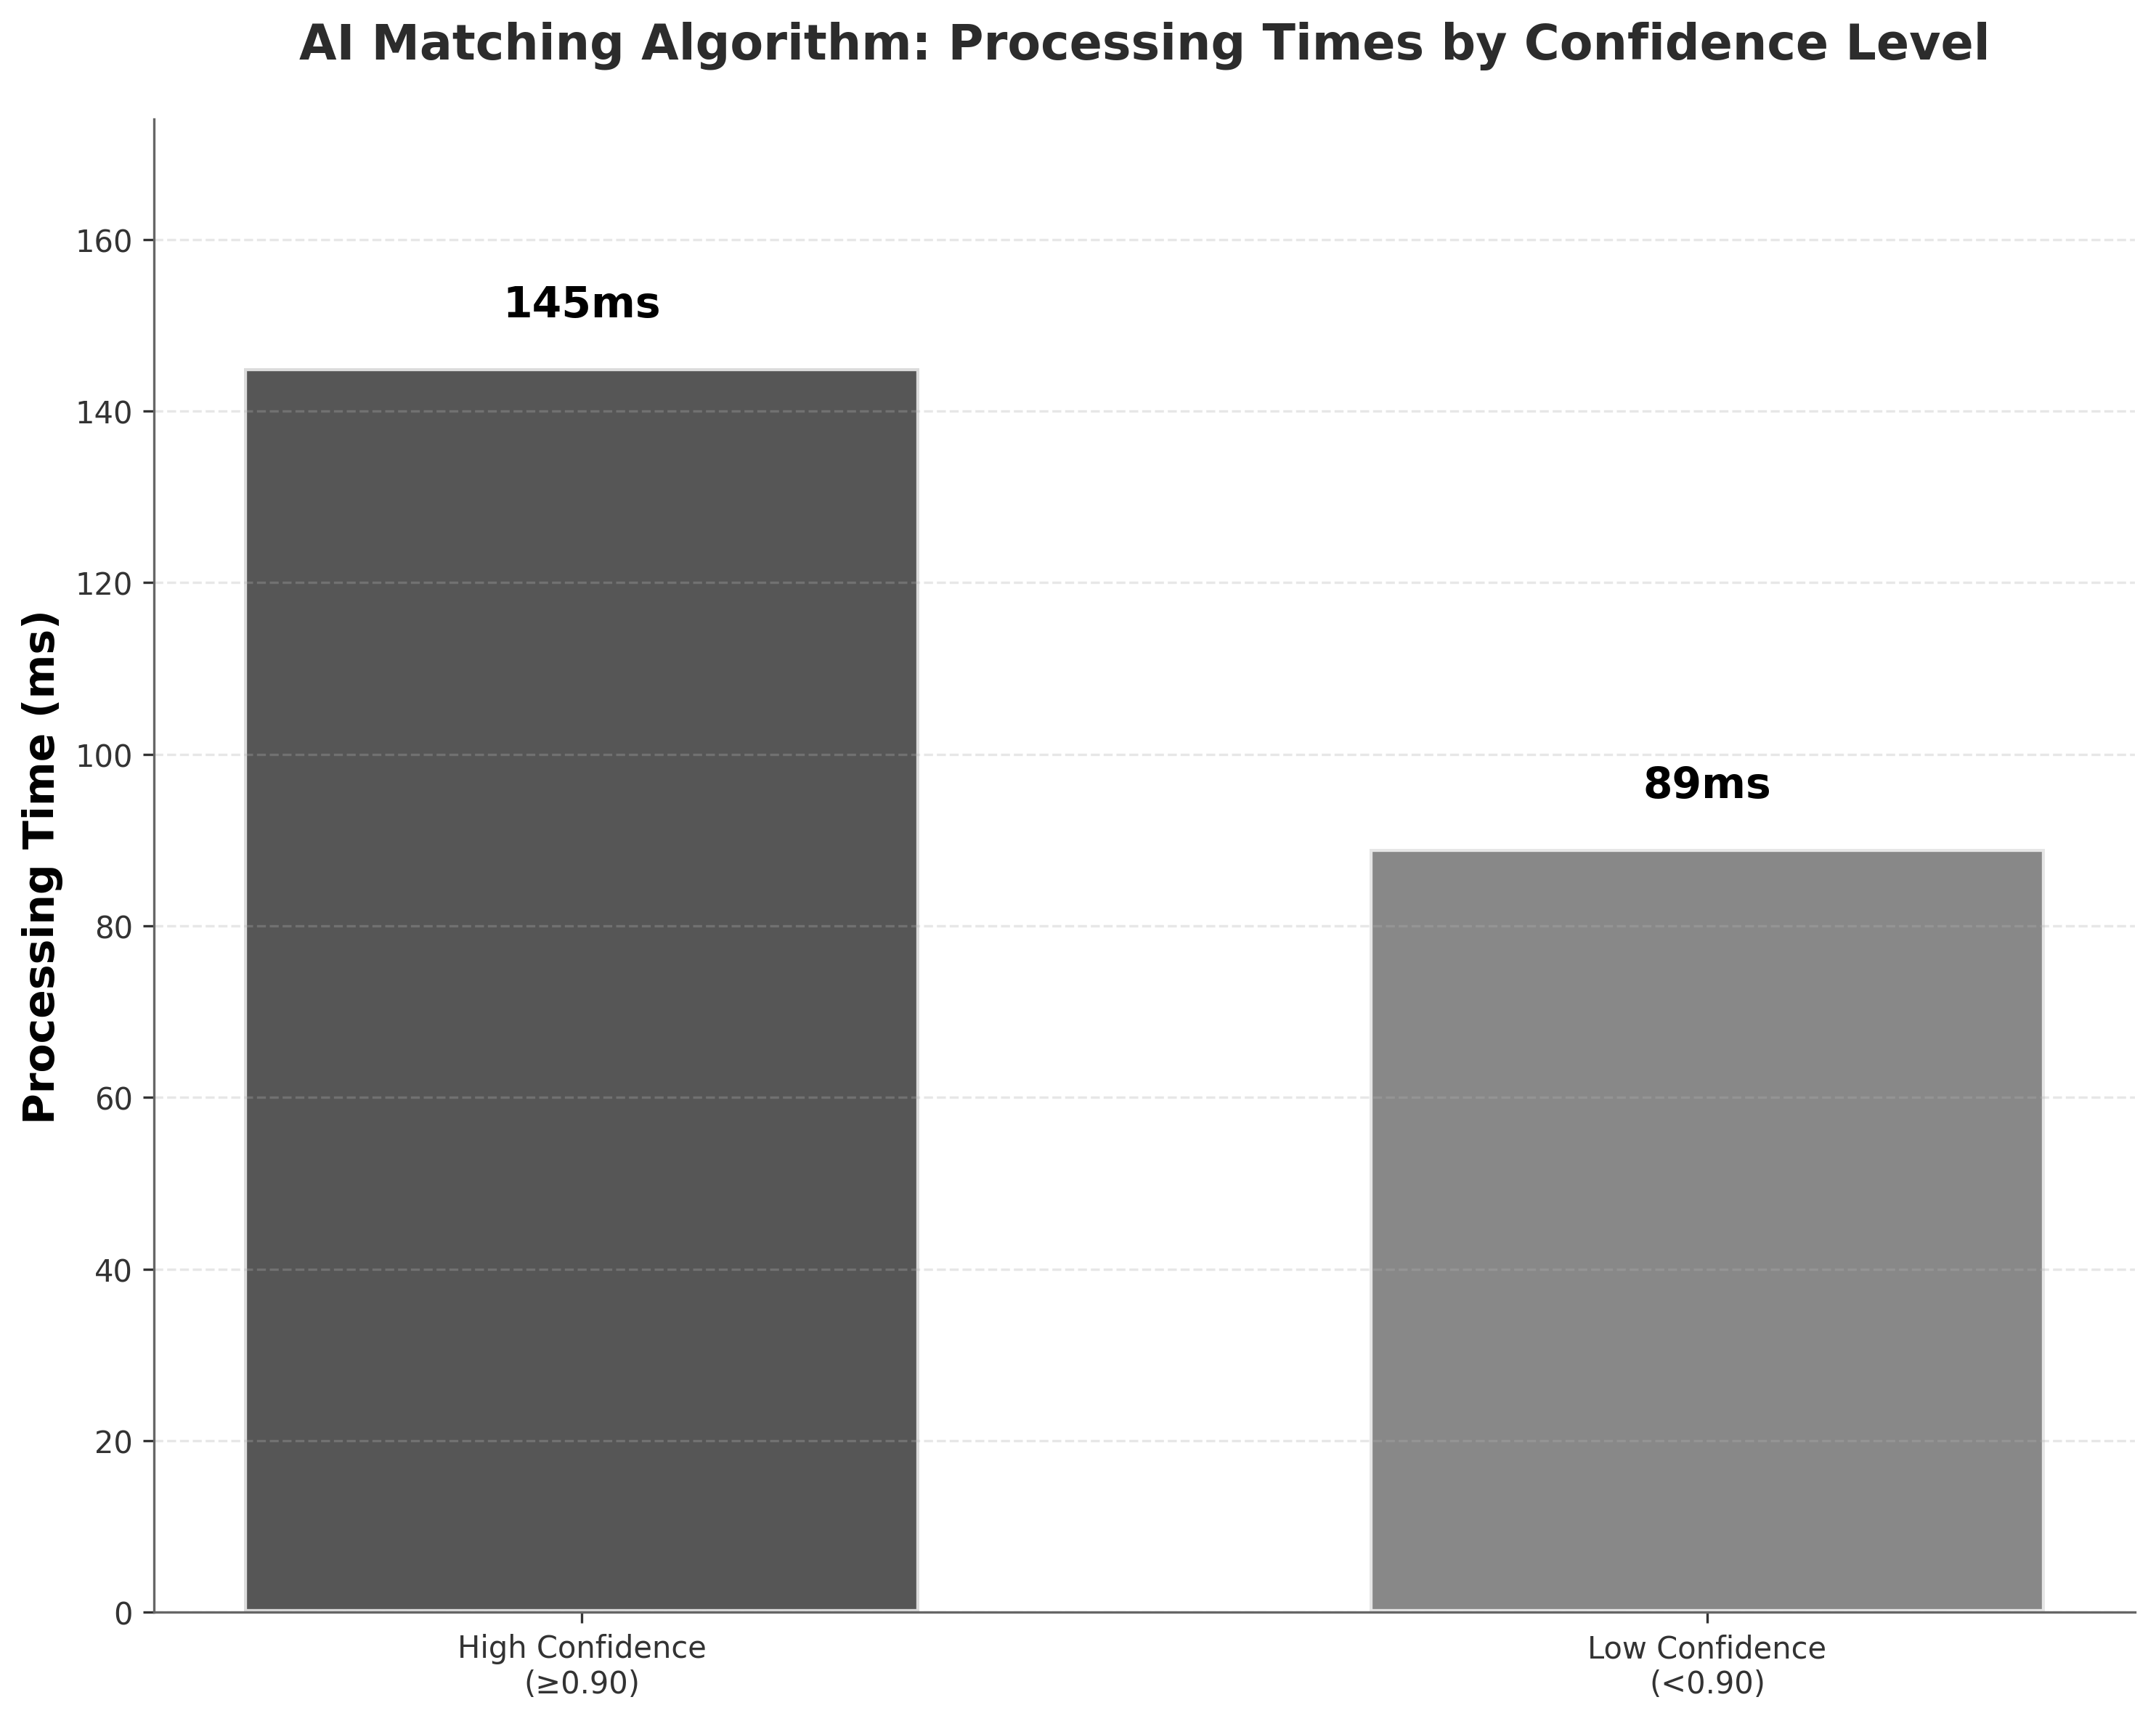
\includegraphics[width=\textwidth]{figs/chapter4/ai_processing_times.png}
        \caption{AI Matching Algorithm: Processing Times by Confidence Level}
        \label{fig:ai_processing}
    \end{subfigure}
    \caption{AI Matching Algorithm Performance Metrics}
    \label{fig:ai_matching_system}
\end{figure}

% TODO: Add sample Grafana dashboard screenshots showing queue monitoring metrics, system health panels, and alert configurations

% ____________________ Frontend Interfaces ____________________ %

\section{Frontend Interfaces} \label{section:frontend_interfaces}

The system provides two distinct user interfaces tailored to different user roles and operational contexts. The web application provides dashboard capabilities for local managers and administrators, and the mobile application enables ordinary users to report and search for lost items in the field.

\subsection{Web Application Architecture} \label{subsection:web_application}

The web dashboard implements a React 19\footnote{\url{https://react.dev/blog/2024/12/05/react-19}} architecture with TypeScript\footnote{\url{https://www.typescriptlang.org/}} for type-safe development and Vite\footnote{\url{https://vitejs.dev/}} as the build tool for optimised development and production builds. The application uses React Router v7\footnote{\url{https://reactrouter.com/}} for client-side routing with nested route protection and Tailwind CSS v4\footnote{\url{https://tailwindcss.com/}} for utility-first styling.

The state management architecture employs React Context API\footnote{\url{https://reactjs.org/docs/context.html}} patterns with four specialised contexts. The component architecture utilises shadcn/ui\footnote{\url{https://ui.shadcn.com/}} component library built on Radix UI\footnote{\url{https://www.radix-ui.com/}} primitives, implementing a compound component pattern for reusable \ac{ui} elements. Advanced table functionality uses @tanstack/react-table\footnote{\url{https://tanstack.com/table/}} for data manipulation, while form handling combines react-hook-form\footnote{\url{https://react-hook-form.com/}} with Zod\footnote{\url{https://zod.dev/}} validation schemas. The system integrates Leaflet\footnote{\url{https://leafletjs.com/}} mapping through react-leaflet\footnote{\url{https://react-leaflet.js.org/}} for geographic visualization and Recharts\footnote{\url{https://recharts.org/}} for data visualization dashboards.

The routing architecture implements protected routes by enforcing authentication before accessing administrative interfaces. The route structure encompasses dashboard overview, inventory management, archived items, delivery points configuration, user management for both managers and regular users, community administration, and system settings.

The complete web dashboard interface showcasing these administrative features and navigation capabilities is presented in Appendix~\ref{app:web_dashboard}, which details the system overview analytics, item distribution management, delivery point performance analysis, community engagement metrics, and category-specific success monitoring.

\ac{api} integration operates through dedicated service modules organised by domain (auth, items, users, managers, points), each implementing \ac{rest}ful communication patterns with the backend endpoint. Token-based authentication persists through localStorage with the automatic refresh mechanisms.

\subsection{Mobile Application Design} \label{subsection:mobile_application}

The mobile application uses Flutter SDK\footnote{\url{https://flutter.dev/}} for cross-platform development with Dart language\footnote{\url{https://dart.dev/}}, targeting iOS, Android, and web platforms. The architecture centres on the GetX\footnote{\url{https://pub.dev/packages/get}} ecosystem for complete state management, navigation, and dependency injection, providing reactive programming patterns and declarative routing.

The \ac{ui} framework implements Material Design 3\footnote{\url{https://m3.material.io/}} principles through GetWidget\footnote{\url{https://pub.dev/packages/getwidget}} as the primary component library, maintaining consistent visual design across platforms. The application structure follows a feature-based organisation with dedicated modules for authentication, community management, item discovery, lost item reporting, delivery points, and user profile management.

State management operates through GetX reactive state patterns with dependency injection via GetX service locator, eliminating the need for context passing and enabling clean separation between business logic and ac{ui} components. Navigation uses GetX's declarative routing system with route guards for authentication-based access control.

\ac{api} integration employs Dio\footnote{\url{https://pub.dev/packages/dio}} \ac{http} client for asynchronous communication with the backend, implementing token-based authentication with secure storage mechanisms for sensitive credentials and local preferences management for user settings.

The feature implementation encompasses community selection and management for multi-tenant access, item discovery with filtering and search capabilities within user communities, lost item reporting with integrated camera and gallery access, delivery point visualisation, and push notification handling for real-time updates. Image handling employs network caching strategies for efficient loading and performance improvements.

% TODO: Add mobile app screenshots showing the main user flows (item reporting, discovery, and matching interfaces)


% ____________________ API Documentation ____________________ %

\section{API Documentation} \label{section:api_documentation}

The framework provides automatic OpenAPI\footnote{\url{https://www.openapis.org/}} documentation generation with interactive \ac{api} exploration capabilities. The documentation includes detailed endpoint descriptions, request and response schemas, authentication requirements, and example usage patterns across all functional modules. Model integration provides schema accuracy with automatic validation rules and constraint documentation.

This interactive interface enables developers and stakeholders to explore \ac{api} capabilities without external tools, supporting authentication testing through Bearer token input and real-time request execution against development and staging environments. Documentation updates automatically with code changes, maintaining consistency between implementation and specification throughout the development lifecycle.

Besides that, throughout the development process, 34+ markdown files were created covering implementation details, architectural decisions, and operational procedures. Code documentation uses inline comments and architectural diagrams for visual system representations, allowing for knowledge transfer, system maintenance, and some possible future development activities.

% ____________________ Deployment Architecture and Operations ____________________ %

\section{Deployment Architecture and Operations} \label{section:deployment_operations}

The deployment architecture coordinates nine containerized services across backend and frontend Docker Compose\footnote{\url{https://docs.docker.com/compose/}} configurations, creating a production-ready environment for system reliability, observability, and maintainability.

\subsection{Containerized Deployment Architecture} \label{subsection:container_deployment}

The deployment architecture coordinates nine containerized services: seven in the backend environment and two in the frontend development environment. On the backend, seven services work in concert - FastAPI serves as the application's core (port 8000), PocketBase handles data storage (internal port 8080, exposed on 8090), and Nginx acts as the reverse proxy (ports 80 and 443). For observability, Prometheus (port 9090) gathers metrics, paired with Grafana (port 3000) for visualization. Node Exporter (port 9100) tracks system health while Nginx Exporter (internal port 9113, exposed on 9114) captures web server statistics. The frontend development environment runs separately, hosting a React application on port 5173 alongside a Flutter web interface on port 8080.

Figure \ref{fig:docker_architecture} illustrates the complete containerized architecture with service dependencies, port mappings, and network isolation between backend and frontend environments.

\begin{figure}[htbp]
\centering
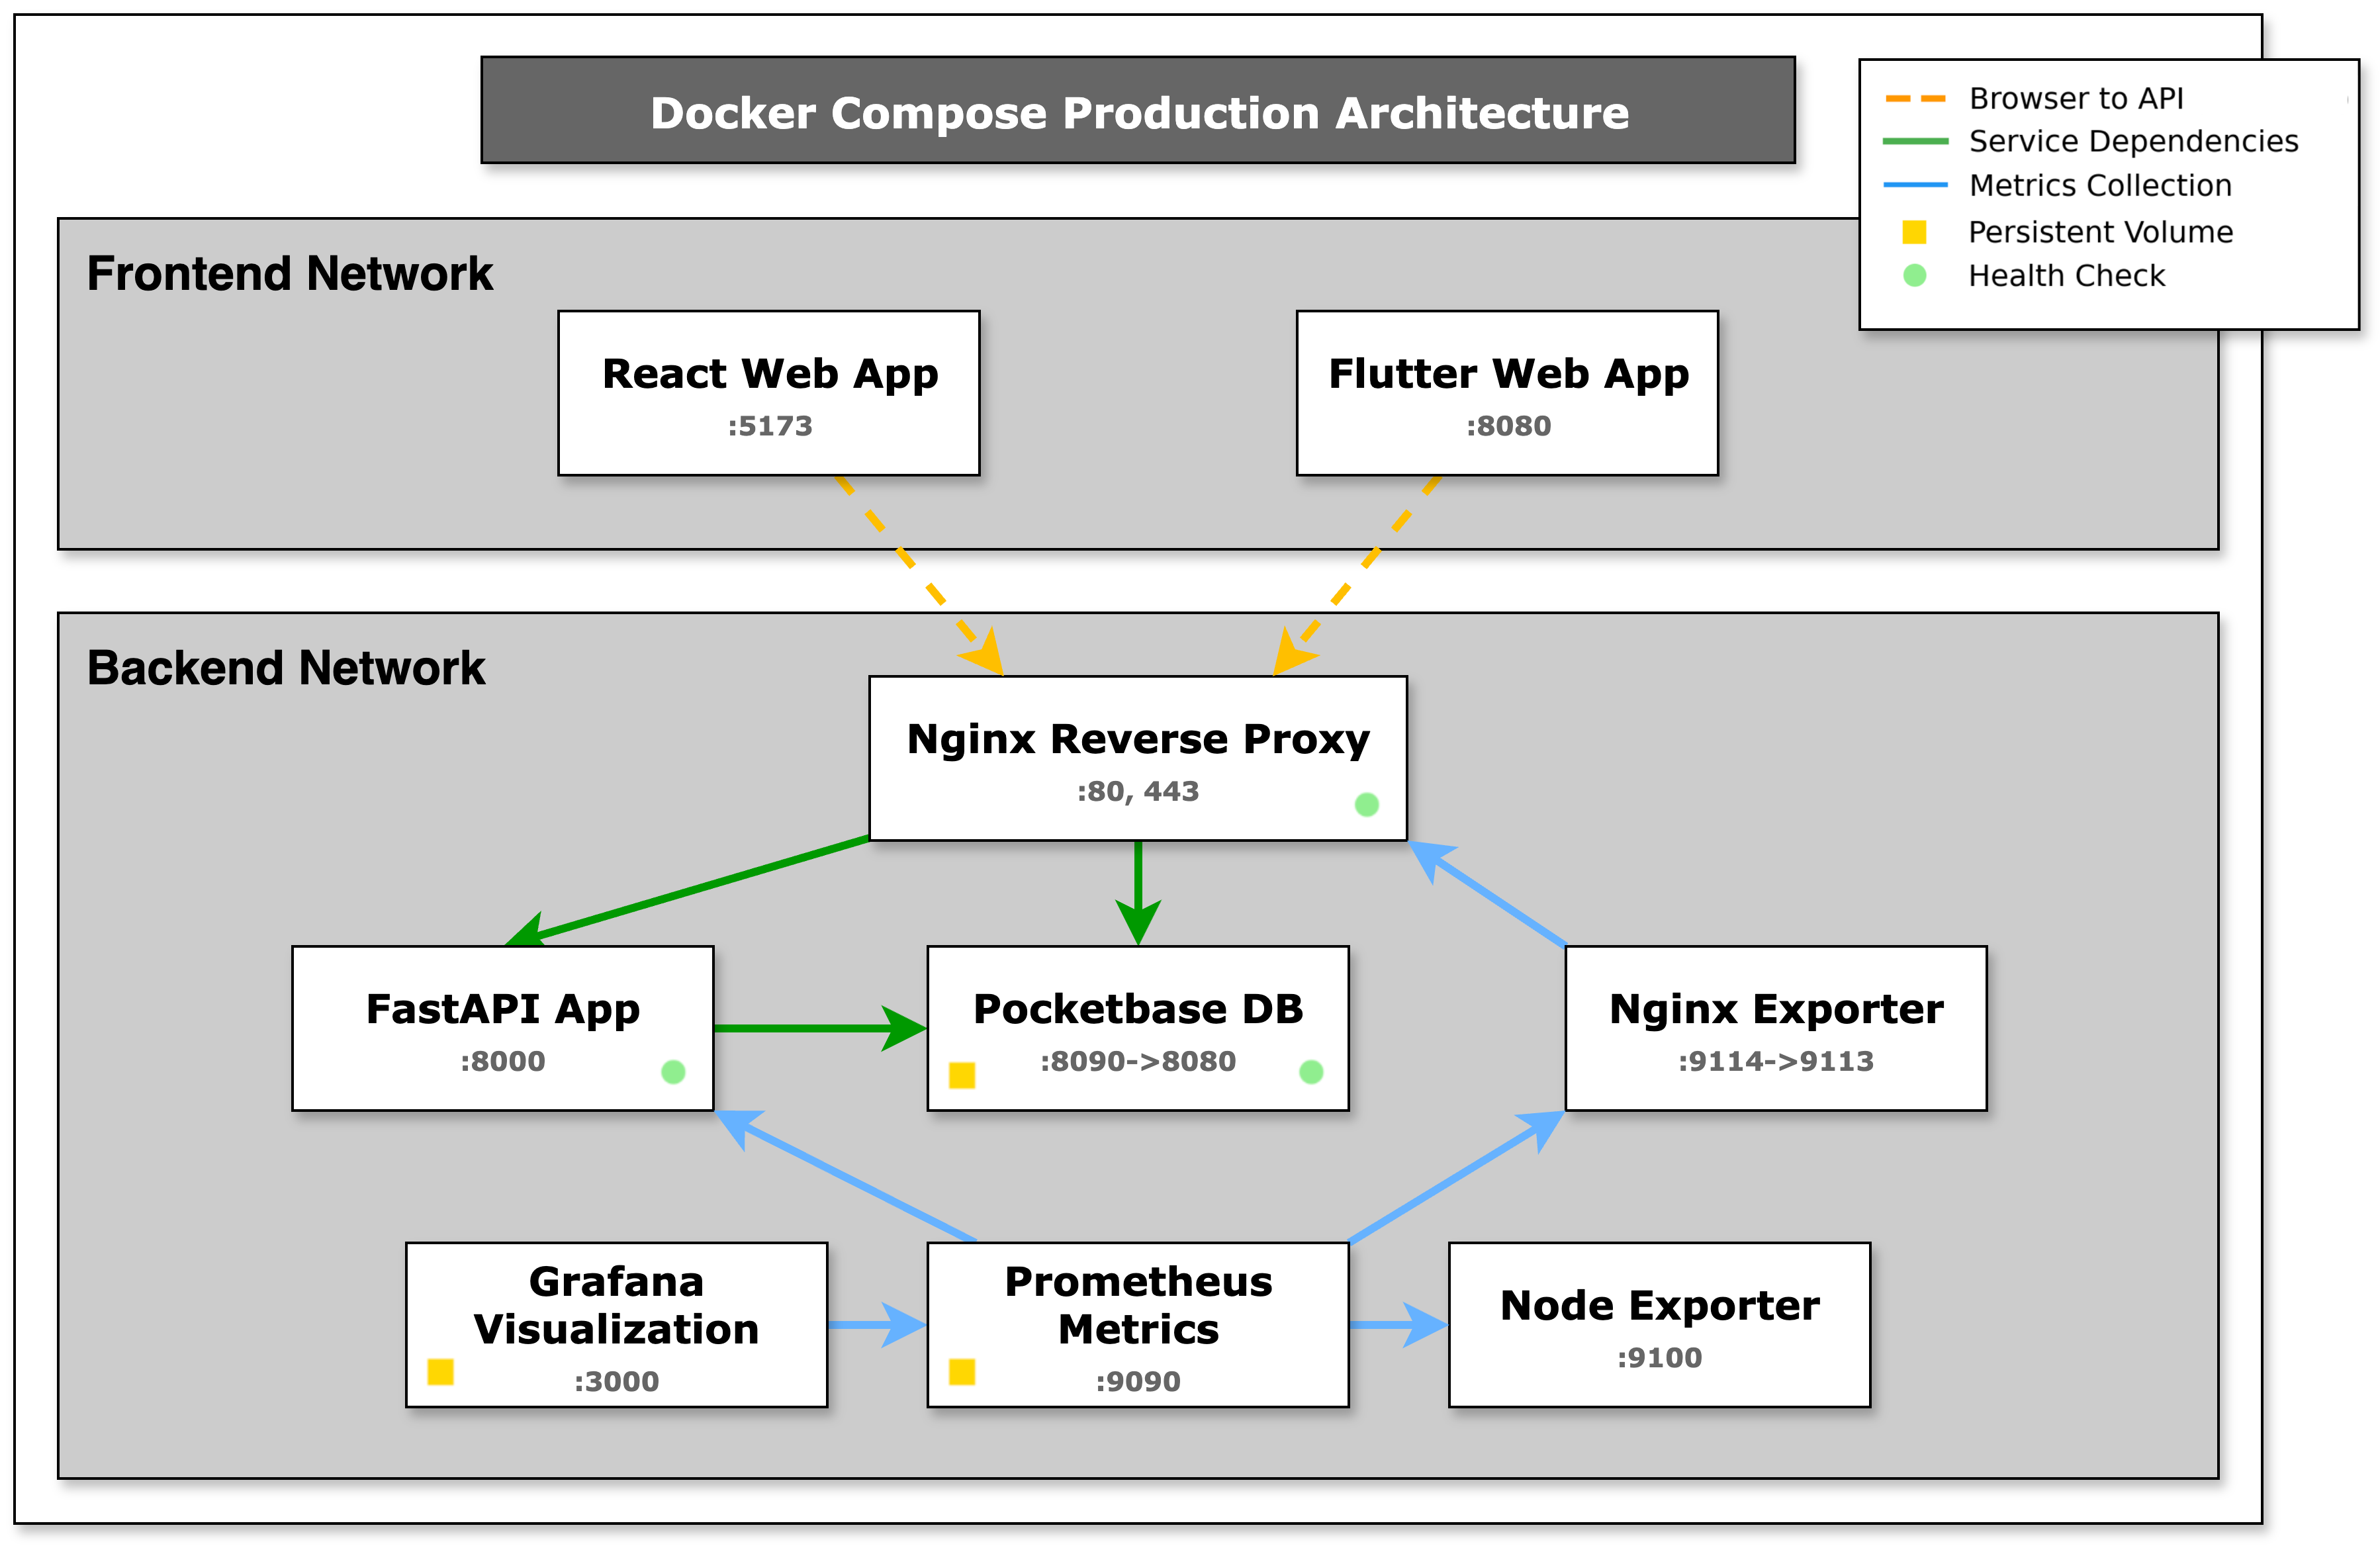
\includegraphics[width=\textwidth]{figs/chapter4/docker_architecture_diagram.png}
\caption{Docker Compose Production Architecture: 9 Containerized Services with Nginx Gateway Routing}
\label{fig:docker_architecture}
\end{figure}

The services connect in a hierarchical dependency chain where FastAPI needs PocketBase to be running, the monitoring stack watches FastAPI, and Nginx waits for both application services before accepting traffic. For system resilience, health checks ping each service's HTTP endpoint at regular intervals - every 15 seconds for PocketBase and FastAPI, every 30 seconds for Nginx. When a service fails these checks, Docker automatically restarts it according to configured policies: \texttt{on-failure} for application services and \texttt{unless-stopped} for the monitoring stack.

Backend and frontend services run in separate Docker Compose stacks with distinct bridge networks (\texttt{backend\_network} and \texttt{frontend-network}). The production architecture routes all \ac{api} traffic through the Nginx gateway, providing centralized security, rate limiting, and request routing. Frontend applications communicate with the backend using \texttt{http://localhost/api}, which the browser resolves to the Nginx gateway on port 80. Nginx then proxies these requests to the appropriate backend services - \ac{api} requests to FastAPI, authentication to specialized endpoints, and file uploads to dedicated handlers. This architecture creates a single entry point for all client traffic, allowing consistent security policies, \ac{cors} handling, and connection pooling. Frontend development servers run on ports 5173 (React) and 8080 (Flutter), serving applications that execute in the browser and communicate with the backend through the Nginx gateway.

Docker volumes handle data persistence, maintaining information safety during container restarts. PocketBase writes to \texttt{pb\_data}, Prometheus saves metrics to its named volume, and Grafana stores dashboards and settings in another persistent volume. Alpine-based images keep container sizes minimal while pinned specific versions in Dockerfiles provide consistent deployments across environments.

\subsection{Monitoring and Observability} \label{subsection:monitoring_observability}

The monitoring infrastructure operates across three layers to capture system visibility. Prometheus scrapes FastAPI's metrics endpoint every 5 seconds, providing application-level insights into request handling and processing times. Docker's built-in metrics track container resource usage and health status across the deployment. For deeper system visibility, Node Exporter reads directly from the host's \texttt{/proc} and \texttt{/sys} directories (mounted read-only for security), capturing per-core CPU usage, memory allocation, disk space, and network traffic.

Grafana transforms these raw metrics into four dashboard views. The system overview tracks CPU, memory, and disk I/O across all services. Application performance dashboards show response times, throughput, and error rates. Business metrics reveal item lifecycles, user activity patterns, and claim resolution statistics. Alert panels highlight when any metric crosses its configured threshold.

Alert rules reside in \texttt{/etc/prometheus/rules}, mounted as a directory in the Prometheus container. A 30-day retention window for metrics provides automatic pruning of old data to prevent disk exhaustion.

\subsection{Operational Procedures} \label{subsection:operational_procedures}

Deploying the system requires coordinating both backend and frontend environments. The backend pulls its configuration from a \texttt{.env} file containing database credentials, \ac{api} keys, and feature flags. Frontend services receive environment variables directly from the Docker Compose file, particularly for development mode settings.

A typical deployment follows three steps. First, \texttt{docker-compose config} validates that all configuration files parse correctly. Then \texttt{docker-compose build} constructs the container images from Dockerfiles. Finally, \texttt{docker-compose up -d} launches everything in detached mode. The system waits for health checks to pass before routing traffic to newly deployed services.

Docker volumes maintain data safety between container restarts and redeployments. PocketBase writes everything to \texttt{pb\_data}, while Prometheus and Grafana each maintain their own named volumes for metrics and dashboards.

System security requires regularly updating the base images specified in Dockerfiles, then rebuilding and redeploying affected services. The 30-day Prometheus retention policy prevents disk space issues by automatically cleaning up old metrics data.

When services crash, Docker's restart policies activate automatically. Application services use \texttt{on-failure} to restart after crashes, while monitoring services run with \texttt{unless-stopped} to maintain availability unless explicitly shut down. If services lose network connectivity to each other, tearing down and recreating the Docker network often resolves the problem - using \texttt{docker-compose down} followed by \texttt{docker-compose up}.

\section{Summary} \label{section:implementation_summary}

This chapter presented the implementation and deployment of the UAchado intelligent \ac{lfms}, demonstrating how architectural decisions from Chapter \ref{chapter:methodology} translated into a functional, production-ready system. The database implementation established a 17-collection PocketBase schema supporting multi-tenant architecture with community-based scoping, hierarchical \ac{rbac}, and optimised query patterns. Core services delivered specialised functionality through FastAPI with 11 routers, implementing authentication with \ac{jwt} validation and caching, complete item lifecycle management with automated security classification, and reverse proxy architecture using Nginx for \ac{ssl} termination and differentiated rate limiting. The \ac{ai} integration employed \ac{llava} through Ollama for multimodal analysis, implementing a multi-factor scoring matching algorithm (description similarity, category alignment, visual comparison, geographic and temporal proximity) and confidence-based thresholds for human-in-the-loop verification.

The system provides asynchronous queue processing with batch management handling over 50 items per minute per community and dual frontend interfaces tailored to distinct user roles. The web application employed React 19 with TypeScript, Context API state management, and shadcn/ui components for administrative dashboards, while the mobile application utilised Flutter with GetX ecosystem for cross-platform field operations. The deployment architecture coordinates nine containerized services through Docker Compose configurations, providing monitoring via Prometheus and Grafana integration, automated health checks and recovery procedures, and operational workflows for configuration management and system maintenance. The complete system includes automatic OpenAPI documentation, markdown documentation covering multiple implementation files, and error handling across all service boundaries.